\chapter{Physically-Informed Uncertainty Models for Spatiotemporality}
\td{Need new intro for this section}


\section{Methodology}
\label{sec:methods}
Key to a physically informed model are the observations available and the model selection itself...\td{pithy introduction to the method here}


\subsection{Plume Detection: Treatment of Robotic Science Sensors}
\label{sec:sensor_models}
The observational data available from AUV \Sentry are continuous measurements from multiple science sensors. These data must first be processed into a data stream the can be used to train the \PHUMES model. In the hydrothermal charting task, there is no single sensor that can be used directly as a proxy for whether a parcel of fluid was hydrothermally derived \autocite{jakuba2007stochastic,preston2022discovering}. This lack of exact sensing is due to the variable values of temperature, chemistry, and particulate matter that persist within a plume structure. In the buoyant stem of a plume, positive temperature anomalies may be several degrees warmer compared to ambient seawater; however in the neutrally-buoyant plume layer, these anomalies may be on the scale of sensor noise (only a few hundredths of a degree). Chemistry anomalies may persist longer within a plume, but are subject to unknown and variable rates of microbial digestion or chemical reaction with the environment. Moreover, some chemical signatures may not specifically fingerprint hydrothermal anomalies, and could be equally indicative of other water-mass mixing events in the deep ocean. Finally, some oceanographic properties (e.g., temperature) vary in the water column as a function of depth, and so data must be detrended with respect to position in the water column. Taken together, the environmental complexity requires developing a sensing strategy that can fuse observations from multiple science sensors onboard \Sentry into a data product that indicates whether the robot encountered hydrothermal plume fluids. 

We elect to process the heterogeneous sensor stream into a binary measurement stream, drawing on the work in \autocite{jakuba2007stochastic}, to indicate whether \Sentry was in a plume or in background seawater\footnote{Access to a binary measurement for plume hunting has long been assumed in related work e.g.,  \autocite{tian2014behavior,saigol2009information}}. For this study, \td{back reference the previous chapter more here} we use a conductivity probe (salinity), temperature probe (temperature), oxidation-reduction potential (ORP) instrument (relative ``reactivity'' of water), optical backscatter (OBS) instrument (turbidity), optode (oxygen), and experimental spectroscopic instruments Pythia \autocite{michel2022gas,Harb:12} and SAGE \autocite{kapit2021dissolved,kapit2021measurement} (dissolved methane) to compute a binary measurement. Sensors are internally logged at variable rates, but interpolated and sub-sampled to a fixed 1 Hz frequency with a shared clock time for the purposes of directly comparing the instruments. Each of these sensors has its own physical characteristics and response to the chemistry of plume water. For example, ORP exhibits a large negative spike when first encountering plume water followed by a slow hysteresis back to a nominal values. Measurements of salinity, temperature, and oxygen are expected to be influenced not only by plume water, but background physical mixing in the ocean; turbidity, ORP, and methane are signals strongly associated with hydrothermalism because they are not persistent in background seawater. To account for the different ways in which sensors respond to plume waters, each sensor is processed individually to detect plume masses in each stream (see \cref{tab:sentry_instruments}). Weights are assigned to each sensor based on their individual reliability for identifying plume water, as determined by the science party and consulted experts in preparation for the research expedition. Observations are then classified as plume water or background water using corroboration across sensors: weighted detections for each sensor are summed together and we use a detection threshold to identify an observation as plume or background. A total corroboration score of 4 or more was used to classify an observation as plume. An example of this sensor applied to real \Sentry detections is shown in \cref{fig:detection_example}.

\begin{table}[h!]
    \centering
    \begin{tabular}{c|p{0.6\linewidth}|c}
        Quantity & Positive Plume Detection Criteria & Weight  \\
        \hline
        Salinity & Detrended practical salinity outside 3 standard deviations of the entire time series & 1 \\
        Temperature & Detrended temperatures above the 75th percentile of entire time series & 2 \\
        ORP & Detections less than -0.005 & 2 \\
        OBS & Optical attenuation above the 75th percentile of entire time series & 2 \\
        Oxygen & Detrended concentrations outside one-hour rolling computation of 3 standard deviations & 1 \\
        Methane & Normalized concentration above 0.3 & 2
    \end{tabular}
    \caption{\textbf{Instruments on AUV \Sentry and the criteria used to identify plume fluids for each instrument.} The weight is used to indicate relative trustworthiness of a plume detection for each sensor, and is used in a corroboration scheme that sums detections across sensors in order to make a final determination on whether an observation location contained a parcel of plume fluid or consisted of background seawater. Detrended data removes depth-related cross-sensitivity from the measurements; for example, temperature is stratified in the deep ocean, so to ignore the impacts of depth changes in the data stream, those effects are removed by ``detrending'' the data stream.}
    \label{tab:sentry_instruments}
\end{table}

\begin{figure} [h]
    \centering
    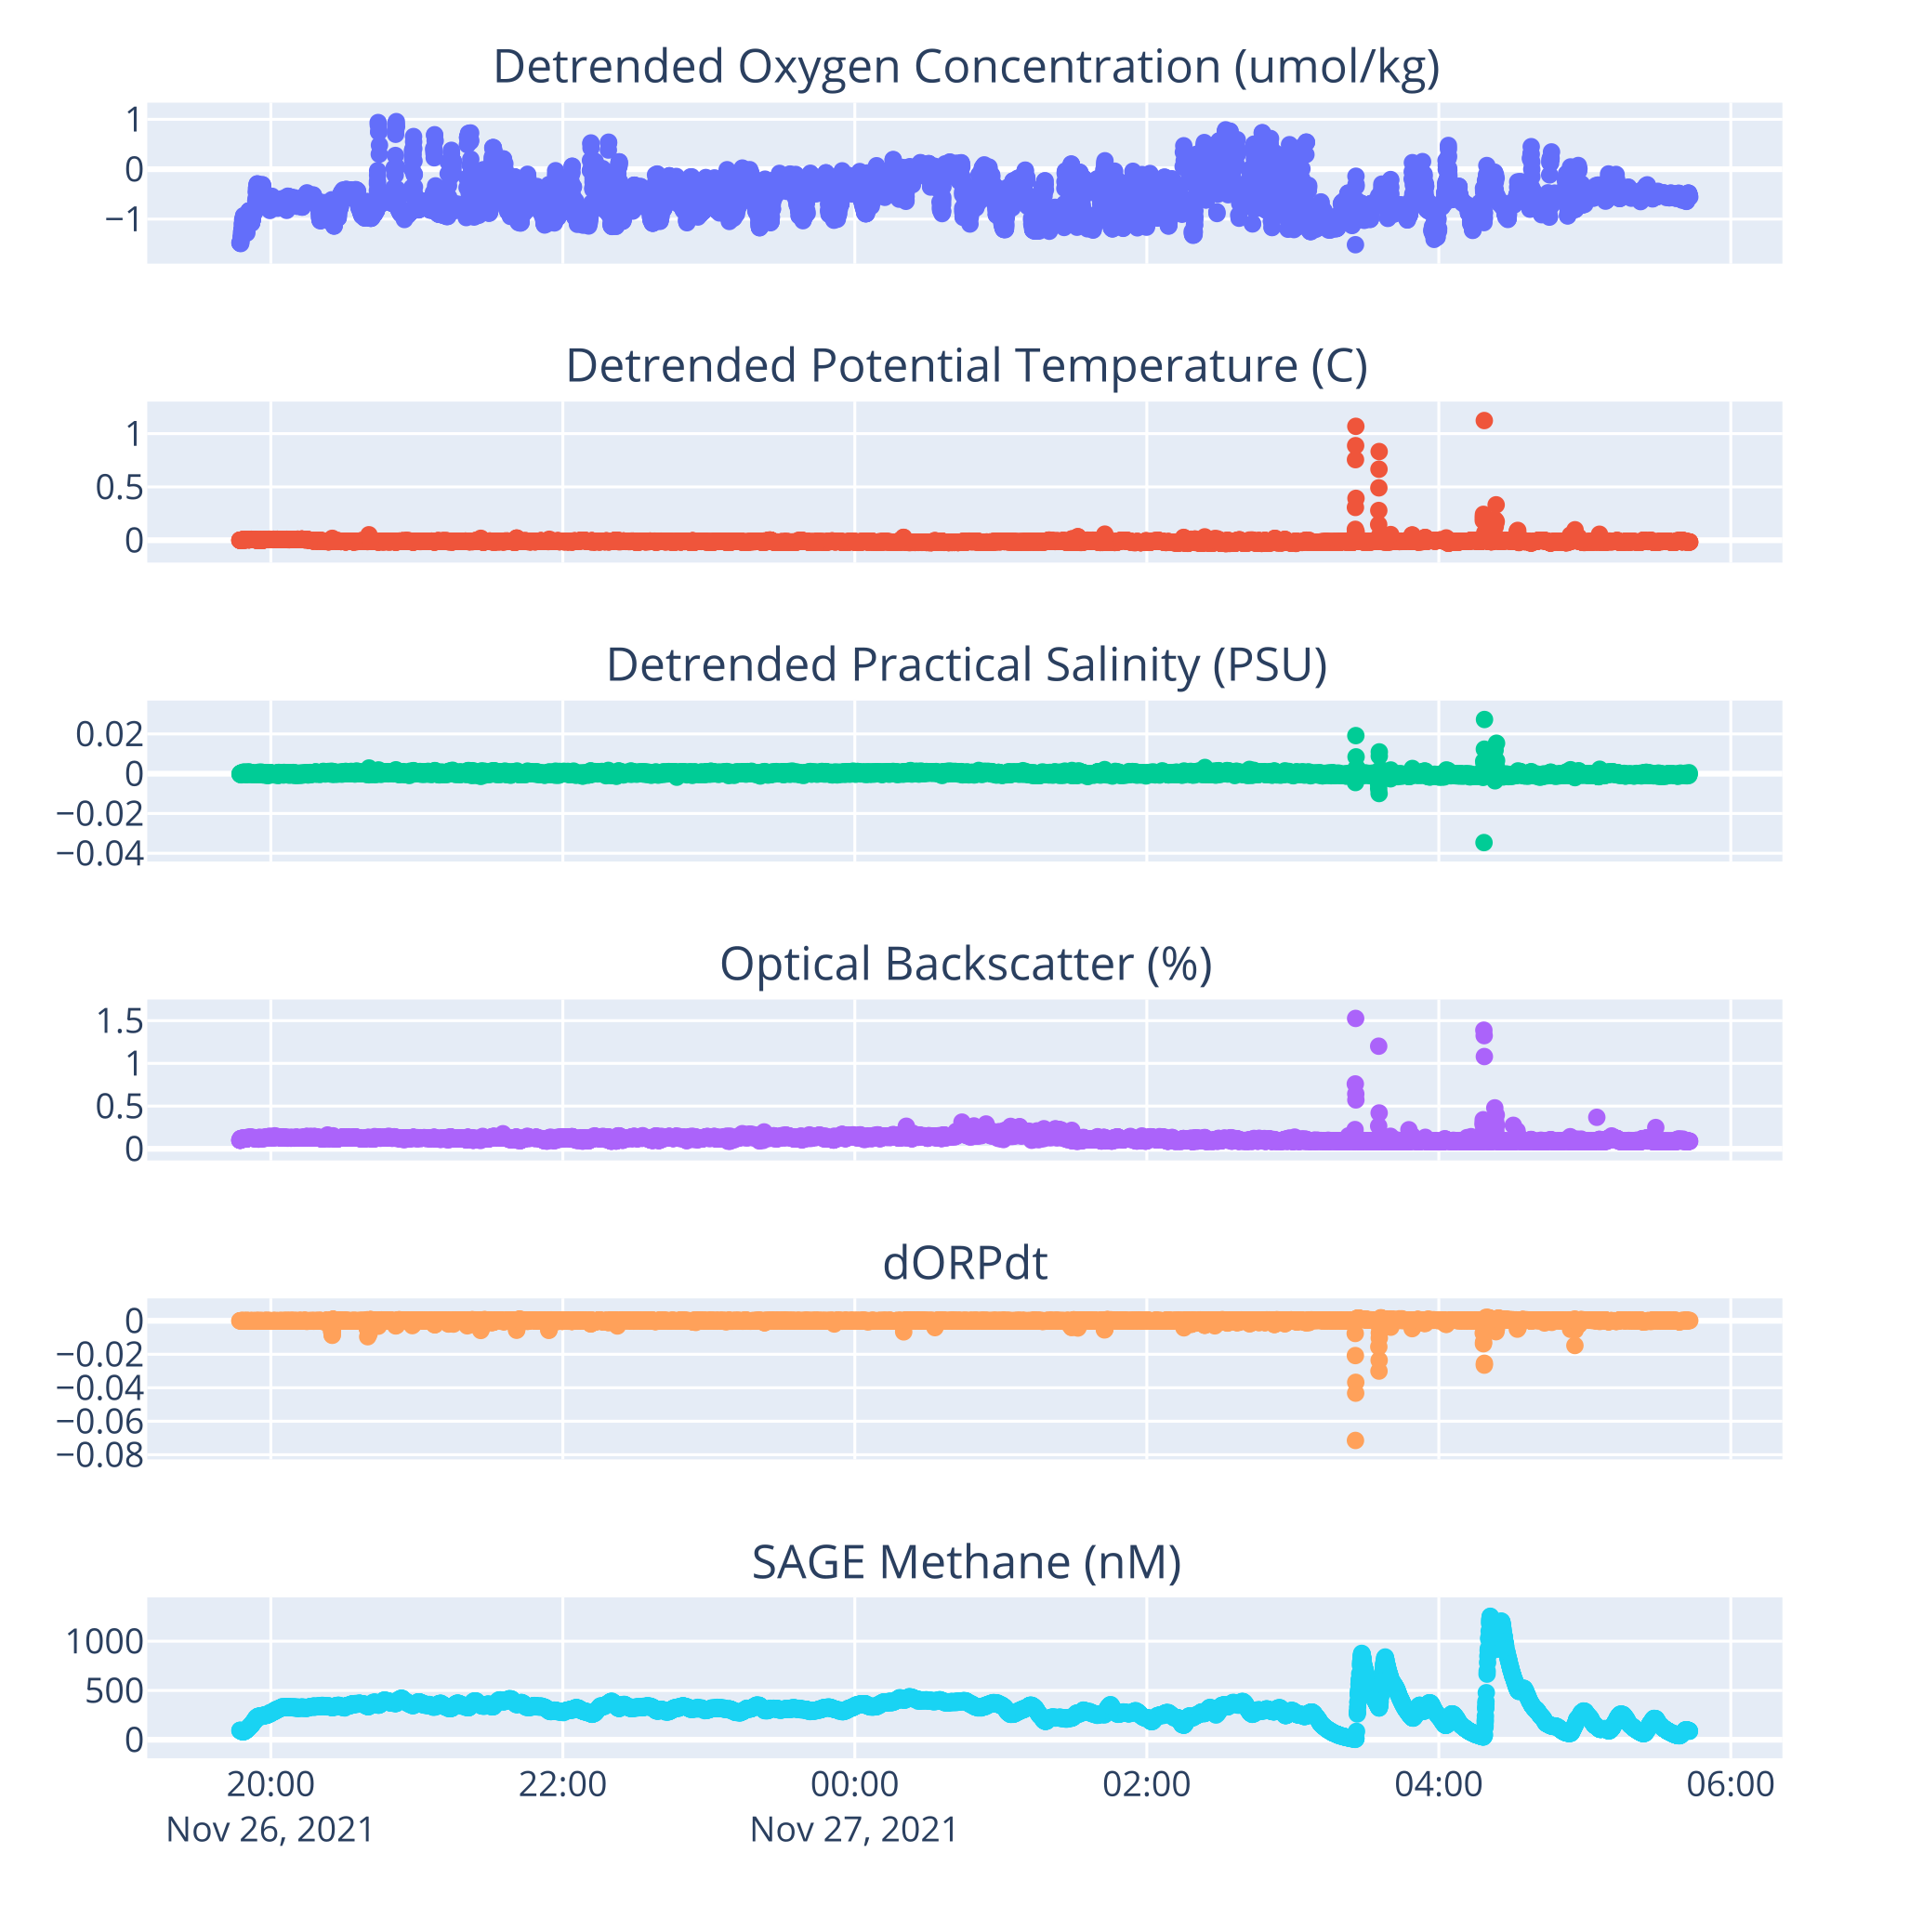
\includegraphics[width=0.45\columnwidth]{figures/binary_example_time.png}
    \hspace{.1in}
    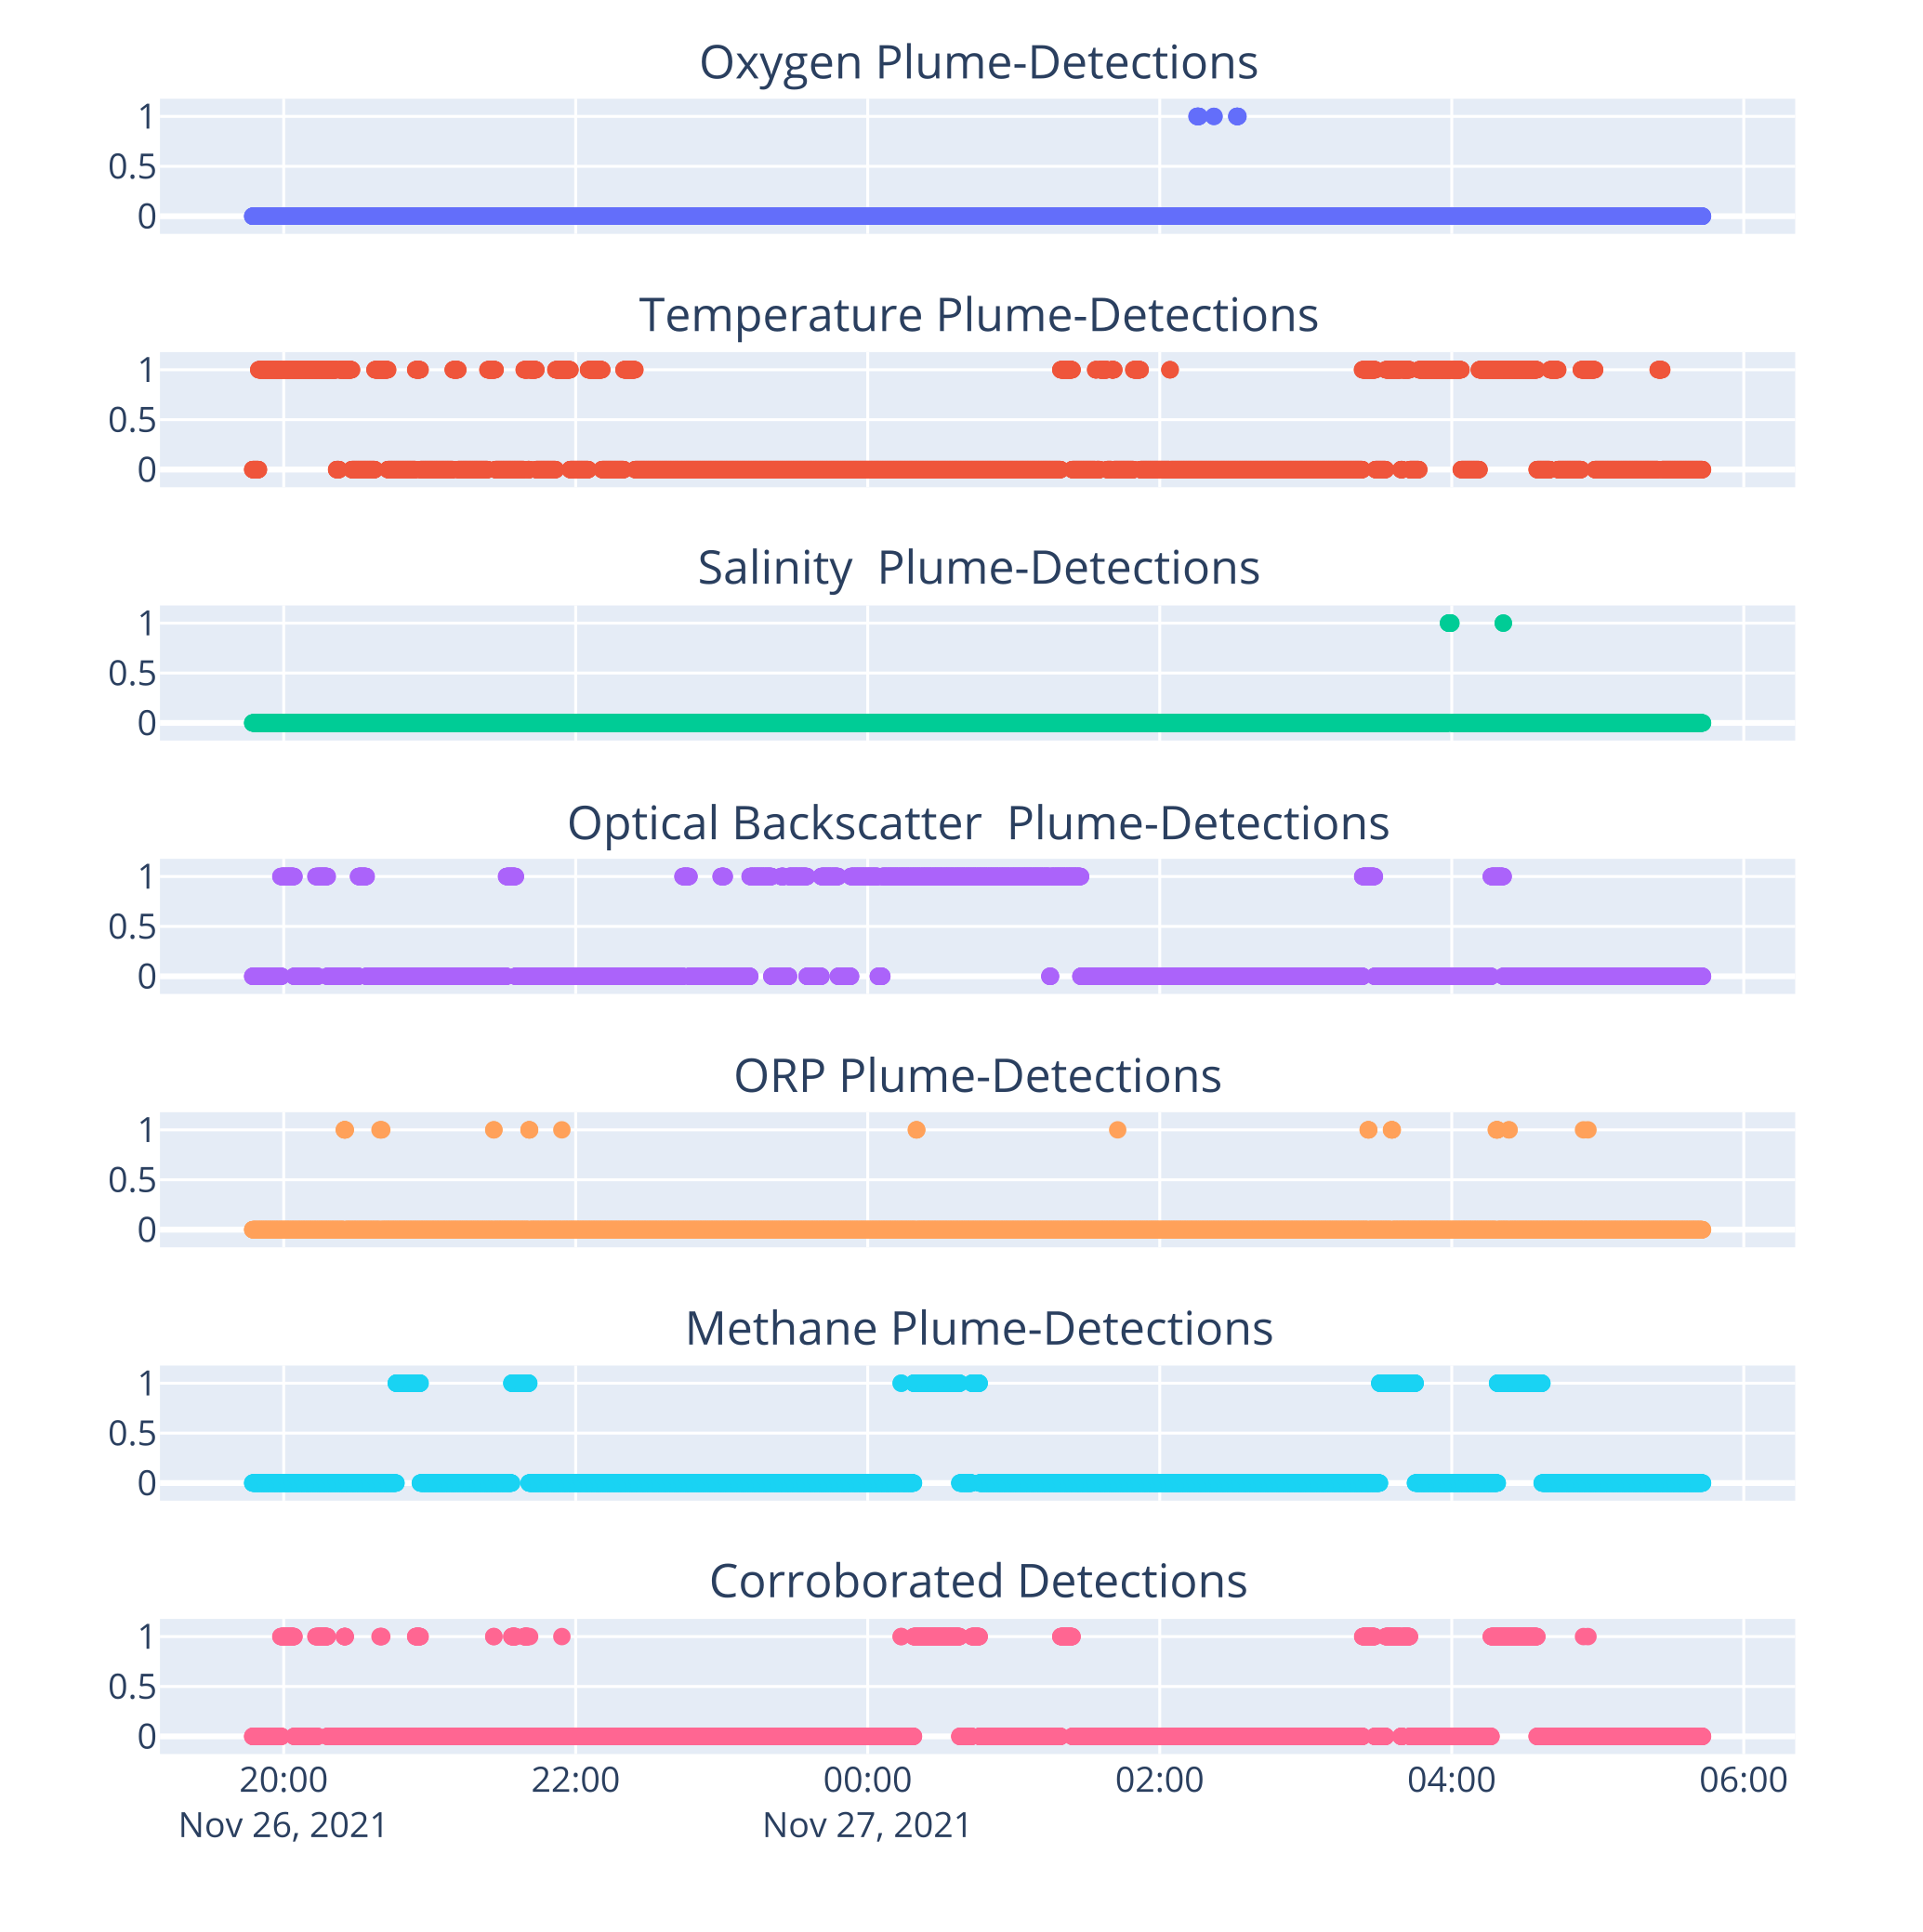
\includegraphics[width=0.45\columnwidth]{figures/binary_example_detections.png}
    \caption{\textbf{Example time series (left) and associated detections (right) over the AUV \Sentry sensor suite.} Oxygen, temperature, and salinity measurements are detrended using a linear transformation fit to depth vs. value plots. The time series demonstrates two types of plume detections. The first are ``obvious detections'' in which most sensors register strong anomalies (this happened twice toward the end of the deployment) and are most strongly associated with buoyant-stem derived fluids. The second are ``persistent-plume detections'' in which the robot traverses through water that is slightly more turbid, warm, or chemical-rich than background water over potentially long horizons (this happened early in the deployment and in the middle). Such detections are most strongly associated with neutrally-buoyant layers. The conservative corroboration detector successfully identifies both forms of plume water.}
    \label{fig:detection_example}
\end{figure}

% This approach for processing complex sensor observations into binary plume detections was initially developed by \autocite{jakuba2007stochastic}; our method is an adaptation of the process using recommendations in this previous work and in consultation with the science team we were directly collaborating with for this study. 
The result of our sensor model is to convert multiple, time-stamped sensor observations $s_{t, i} \in \R, \, i = 1, \dots, S$ to a time-stamped binary plume-detection $z_{p, t} \in \{0, 1\}$. These binary plume detections are then used to update our plume model and plan robot trajectories, as described in the following sections. The accuracy of this sensor model is currently uncharacterized, as there is no available ground truth in a field setting by which to verify the assigned classifications. Qualitatively, the classifications were reviewed by the science team and verified for their alignment with expert opinions on which label to assign.


%%%%%%%%%%%%%%%%%%%
% External Sensing 
%%%%%%%%%%%%%%%%%%
\subsection{External Sensing: Leveraging All Available Information}
\label{sec:external_current}
We deployed several sensing packages during the research cruise to collect relevant information about the state of temporally evolving crossflow $\x_c$ and ambient seawater properties. We leverage these external measurements within our \PHUMES instance in two ways. First, we characterize the background seawater stratification near a target site using a ship-board rosette\footnote{A rosette is often a metal frame on which oceanographic sensors and a carousel of water sampling containers are mounted. It is attached to a ship via a cable, and can be lowered and raised via a winch in vertical transects of the water column, or can be towed by a moving ship horizontally through the water column.} which takes vertical profiles of the water column. The empirical stratification function for Guaymas Basin is used within the physically-informed layer of \PHUMES and treated as a constant throughout the expedition. Second, we learn the crossflow transition function $T_c$. Critically there was no sensor on \Sentry during our expedition that could be used to measure the \emph{in situ} current magnitude and heading. While it may be possible to estimate $T_c$ solely from the binary observations of the plume, access to an external bottom-mounted tiltmeter on the seafloor during this expedition significantly relieved the burden of this inference process. These auxiliary sensors are introduced and discussed in detail in \cref{sec:field_description}. 

% For the former (1), measurements from a temperature and salinity sensor mounted to a ship-board rosette were used to define the depth-dependent density, temperature, and salinity stratification curves of the field site (Guaymas Basin) water column. The stratification curve is a function that describes the changes in density over depth in the ocean, and has implications for how a hydrothermal plume will interact with background seawater. 

% We learn $T_c$ (or, more precisely, the function $h$ by which $T_c$ is defined) by fitting a Gaussian process (GP) with composite radial-basis-function and periodic kernel functions to point observations of crossflow magnitude and heading observed by the tiltmeter. Approximately 3 days of observations were available for training. Crossflow parameters $\x_c$ in $\Ss$ were set with the expected mean of the trained GP. At present, a crossflow sensor is in development for \Sentry using existing acoustic technology onboard the robot; in such a configuration, estimating $T_c$ could be done simultaneously with the plume-charting task.

% PHUMES
\subsection{\PHUMES: Physically-informed Probabilistic Forecasts}
\label{sec:phumes}
\PHUMES is a modeling approach that can generate predictions of the distribution of a spatiotemporally evolving state from a history of sparse state-space observations. To quickly learn a predictive model of a spatiotemporal phenomenon, \PHUMES leverages access to analytical scientific simulators (when available) codified as systems of ordinary differential equations (ODEs). These simulators reduce the dimensionality of the inference problem from the full-state of the environmental phenomenon (e.g., a 4D volume in space and time with binary phenomenon measurement) to the dimensionality of the initial conditions and parameters of the simulator (which can then be used to populate the full-state for planning purposes). The use of ODE systems, as opposed to high-fidelity numerical simulators using partial differential equations (PDEs), is intentional; the computational requirement of most PDE systems used to model environmental phenomenon at the scales studied during expeditionary missions is intractable. In contrast, ODE systems are less well-resolved, but summarize the structure of an evolving phenomenon in a useful way for positioning a robot to encounter plume fluids and that can be enhanced by a generic probabilistic formulation wrapping the ODEs.

For hydrothermal plume charting, we use a time-averaged model of buoyant plume evolution through a weakly stratified fluid under crossflow as described in \autocite{tohidi2016highly} with modifications for seawater as adapted from \autocite{xu2012deep}, which for notational simplicity refer to as function $f(\cdot, \cdot)$. The crossflow ``bends'' the buoyant stem of the plume, and reduces the effective rise height of the plume by introducing more mixing. Using a modified cylindrical coordinate system in which $s$ represents a point along the axis described by the plume centerline and $\theta$ describes the vertical angle from the base of the plume, our \PHUMES simulator takes the form:

\begin{equation}
    \frac{dQ}{ds} = Q\sqrt{\frac{2(1+\lambda^2)}{M\lambda}}(\alpha|\frac{M}{Q} - U_a\cos\theta| + \beta|U_a\sin\theta|)
\end{equation}
\begin{equation}
    \frac{dM}{ds} - U_a\cos\theta\frac{dQ}{ds} = \frac{FQ}{M}\sin\theta 
\end{equation}
\begin{equation}
    U\sin\theta\frac{dQ}{ds} + M\frac{d\theta}{ds} = \frac{FQ}{M}\cos\theta
\end{equation}
\begin{equation}
    \frac{dF}{ds} = -QN^2\sin\theta
\end{equation}
\begin{equation}
    x_a = \int_0^s\cos\theta ds
\end{equation}
\begin{equation}
    h_a = \int_0^s \sin\theta ds
\end{equation}

where $U_a = U_a(z)$ is the ambient crossflow velocity, $Q = Q(s,\theta)$ represents the plume specific volume flux, $M = M(s, \theta)$ is the specific momentum flux, $F = F(s, \theta)$ is specific buoyancy flux, $N$ is the Brunt-V\"ais\"al\"a frequency, $\lambda$ is the ratio of the minor and major axis that define the plume cross-sectional ellipse, $x_a$ and $h_a$ represents the Cartesian transform of $s$ and $\theta$ within the plume's frame of reference, and $\alpha$ and $\beta$ are vertical and horizontal entrainment coefficients. To convert abstract notions of buoyancy and momentum flux to more readily interpretable and observable vent characteristics (e.g., vent area, fluid exit velocity), we can use the following relationships:

\begin{equation}
    Q_0 = \lambda u_0 \frac{A_0}{\pi}
\label{eq:heat_flux}
\end{equation}
\begin{equation}
    M_0 = Q_0 u_0
\label{eq:momentum_flux}
\end{equation}
\begin{equation}
    F_0 = g10^{-4}(T-T_0)Q_0
\label{eq:buoyancy_flux}
\end{equation}

\noindent where $A_0$ is the vent area, $u_0$ is the initial fluid velocity leaving the vent, $T$ is the temperature of fluid at the vent, and $T_0$ is the temperature of ambient seawater at the depth of the vent (note that temperature is the dominant component of density, $\rho$, for deep-sea hydrothermal plumes). Indeed, temperature, area, and exit velocity compose a sufficient set of parameters for representing the initial conditions of any particular plume and plume envelope calculation; these quantities, in addition to the mixing coefficients, form our set of $\x_p$ in $\Ss$ in the plume-charting POMDP. Correspondingly, $U_a$ and the global heading of the crossflow, $\Theta_a$ (not directly modeled in these equations, but can be trivially applied to $x_a$ and $x_h$ to convert plume-reference coordinates to global coordinates), form the parameters in $\x_c$ in $\Ss$.

With the simulator defined, we can now pose a specific inference problem: from observations of plume or background waters, what are the generating initial conditions (vent area, vent fluid temperature, vent fluid exit velocity) and seawater properties (horizontal mixing coefficient, vertical mixing coefficient, global current heading, and global current magnitude)? This allows us to place probability distributions over $\x_p$ and $\x_c$, over which we initially place an uninformative prior, $\Pi(\x_p)$ and $\Pi(\x_c)$ and aim to learn the posterior distributions $\Pi(\x_p | \Zz)$ and $\Pi(\x_c | \Zz)$ \footnote{We effectively separate inference over $\x_p$ and $\x_c$ given the observation model available; indeed we assume that observations of crossflow can be treated as independent of observations of plume detections. This is strongly supported in the practical deployment of \Sentry, when an external sensor was necessary to observe crossflow. If instead the sensors were co-located on \Sentry, inference over the joint posterior $\Pi(\x_p, \x_c | \Zz)$ could be done instead.}.

\begin{figure}[h!]
    \centering
    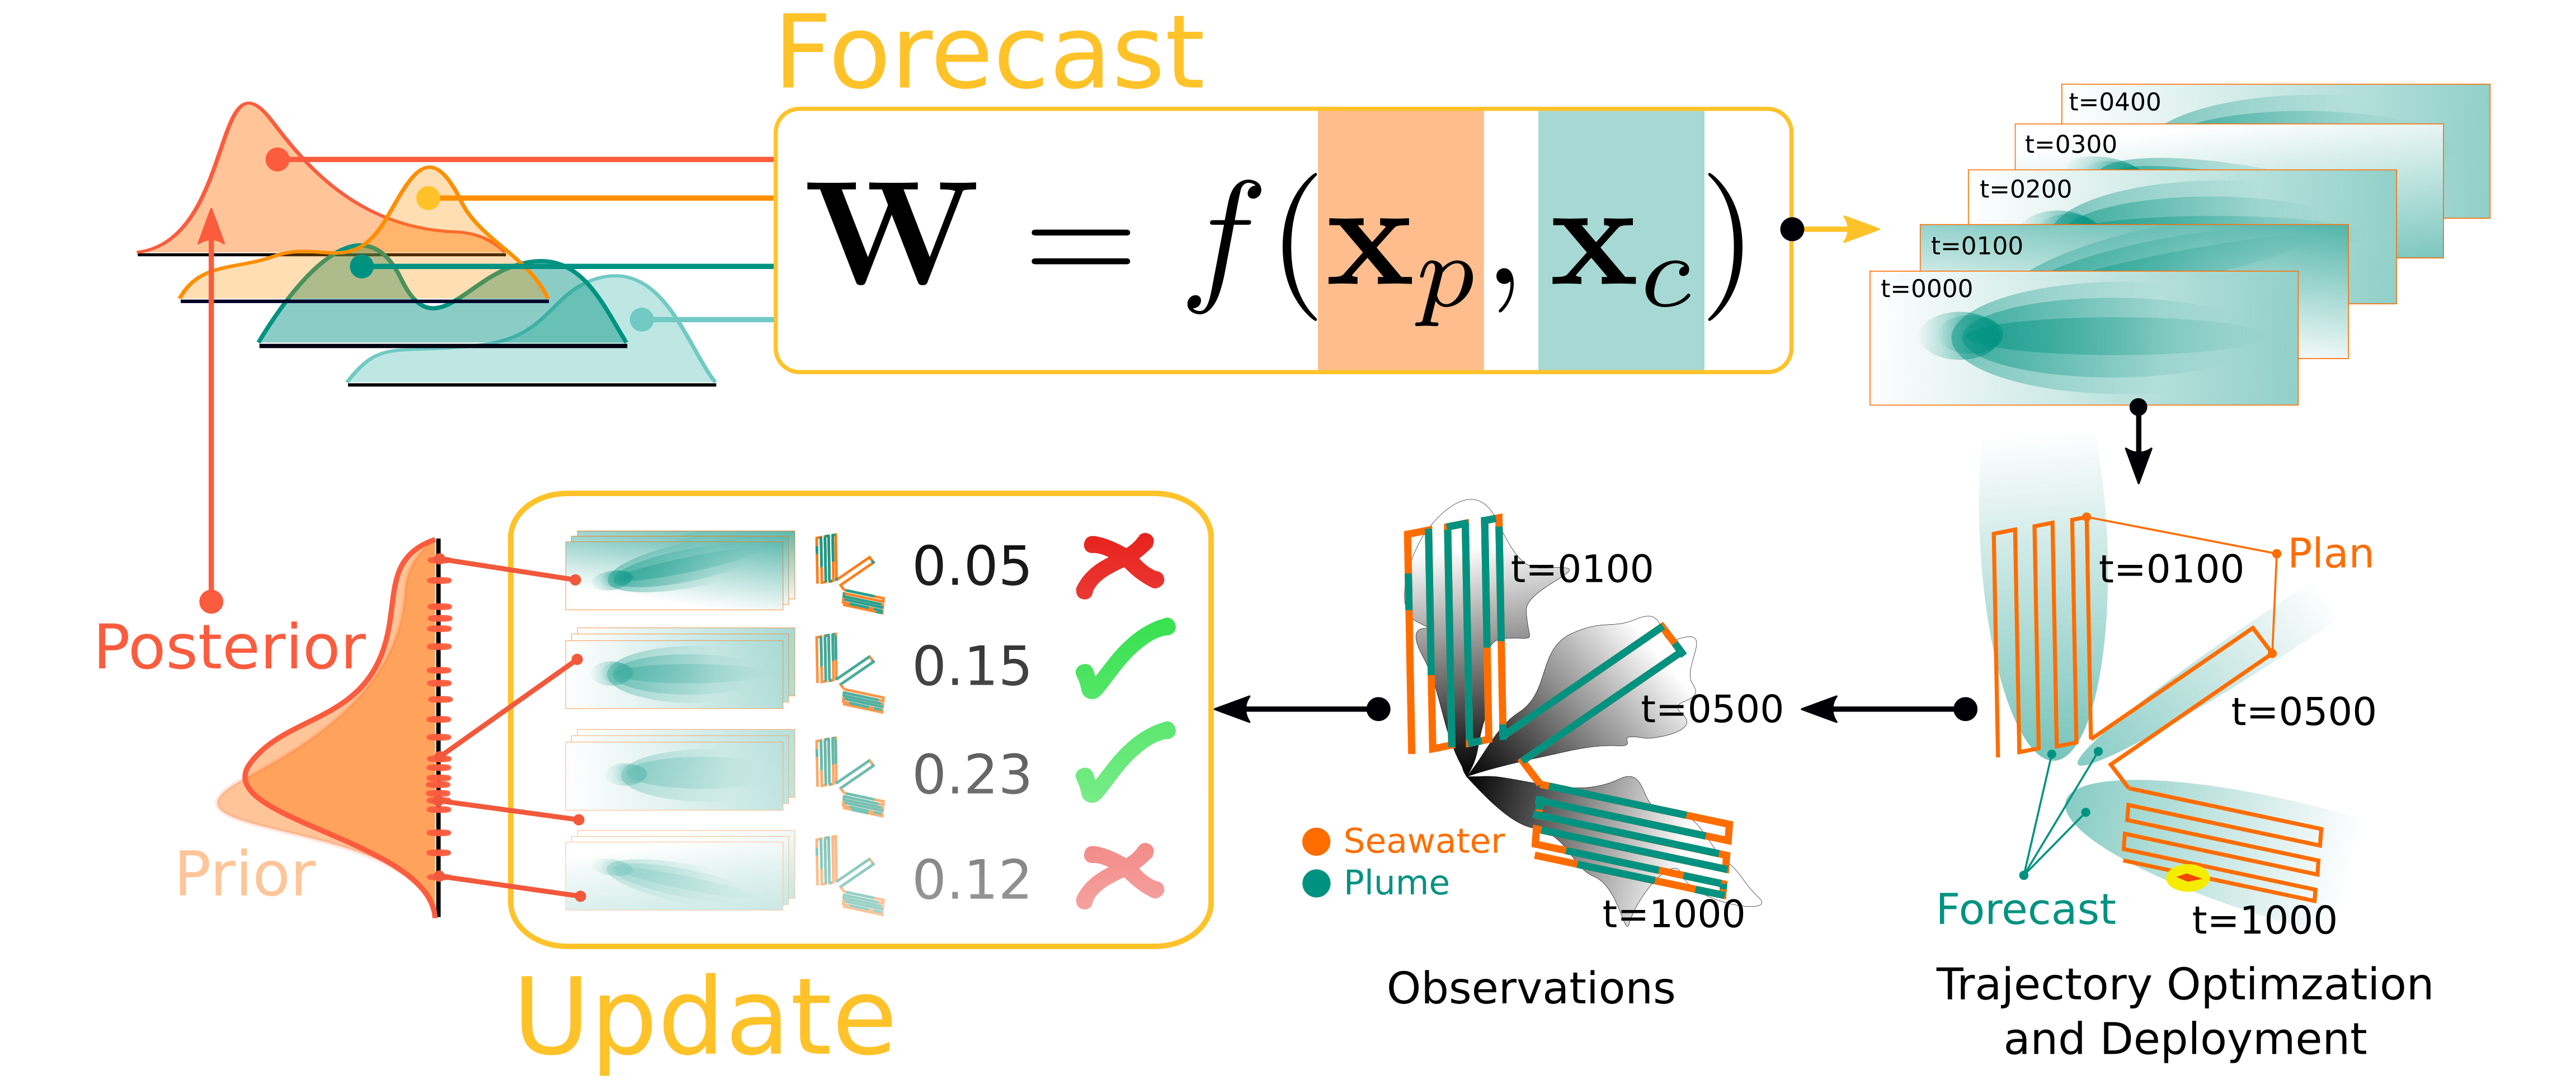
\includegraphics[width=1\columnwidth]{figures/phumes_diagram.png}
    \caption{\textbf{\PHUMES}: \phumes. \PHUMES is a model for forecasting the evolution of a spatiotemporal distribution trained on partial observations. \PHUMES generates forecasts by leveraging an embedded analytical model $f(\cdot, \cdot)$ that approximates the physics-driven evolution of a target distribution. This model is seeded with many samples from distributions placed over initial conditions, physical parameters, or temporal functions (such as $\x_p$ and $\x_c$ here). The composite result of this process is a forecast $\mathbf{W}$ that consists of a mean and variance of phenomenon occupancy in a 3D volume over snapshots of time. This forecast is provided to a trajectory optimizer which sets a deployment trajectory that is executed by a robot. The deployment generates a series of observations, which are then used to update the distributions of the generating distributions via MH-MCMC, which compares the gathered observations with the simulated observations of samples from the generating distributions. The resulting posterior update over the generating distributions is then used for the next planning iteration.}
    \label{fig:phumes}
\end{figure}

\PHUMES consists of two key phases: forecasting (forward simulation) and updating (inverse problem) (\cref{fig:phumes}). In the forecasting step, samples from the distributions of the initial conditions and seawater properties seed the simulator which is solved many times to create a set of plume-envelope samples in the full state space of the target phenomenon (and trajectory optimizer). Time is discretized over domain-specific key points, and any parameters reliant on time are sampled at those discrete points. The set of composite samples at each time is a ``forecast'' that is essentially a series of snapshots of the phenomenon. Precisely, \PHUMES generates a time-indexed $t \in \mathbb{T}$ composite estimate of the distribution of plume fluid in a 3D volume $\overbar{\mathbf{W}}$ by forward simulating time-dependent $M$ samples of the states $x_{p,t}^{(m)} \sim \Pi(\x_p(t))$ and $x_{c,t}^{(m)} \sim \Pi(\x_c(t))$ through the plume simulator $f(\cdot, \cdot)$:

\begin{equation}
    \overbar{\mathbf{W}}_t = \frac{1}{M}\sum_{m=1}^{M} f(x_{p,t}^{(m)}, x_{c,t}^{(m)}) \hspace{1cm} \forall t \in \mathbb{T}.
\end{equation}

The complete forecast $\overbar{\mathbf{W}}_t$ is then used by a trajectory optimizer to approximate the reward function $R([\x_p, \x_c, \x_r]^T, a) = \indic{\texttt{in\_plume}(\x_p, \x_c, \x_r, a)} \approx \indic{\texttt{in\_plume}(\overbar{\mathbf{W}}, a)}$. Equivalently, $\mathbf{W}$ is the robot's belief $b$, and as it consists of a set of samples, any statistical measure (the maximum \emph{a posteriori} estimator (MAP), maximum likelihood estimator (MLE), median, etc.) can be computed. For instance, the variance of the forecast $\mathbf{S}^2_W$ can be computed and used within an information-theoretic reward function (e.g., upper confidence bound), as contingent on the design of a downstream planner. 

After the trajectory optimizer yields a plan, \Sentry is deployed. For a single deployment, upwards of 20,000 observations may be available (each deployment is a minimum of 6 hrs in duration, up to 24 hrs, and sensor measurements are logged at 1 Hz). Using the filter described in \cref{sec:sensor_models}, AUV \Sentry provides observations of binary plume detections. Other sensors of opportunity described in \cref{sec:external_current} provide continuous crossflow magnitude and heading observations. These observations are collated into the sensor model $\Zz$.

At the update step of \PHUMES, the probability distributions over $\x_p$ and $\x_c$ are updated from observations $\Zz$. To find $\Pi(\x_c|\Zz)$ we use GP models for crossflow magnitude and heading as described in \cref{sec:external_current}. The GP kernel parameters are updated using a maximum-likelihood update following typical procedures \autocite{Rasmussen2004}. For $\Pi(\x_p | \Zz)$, we use a random-walk Metropolis-Hastings Markov Chain Monte Carlo (MH-MCMC) method \autocite{metropolis1953equation} to perform the update. Simulations of deployments are generated by solutions to the numerical model $f(\cdot, \cdot)$ seeded with samples from $\x_p$ and $\x_c$. The output of the simulations is directly compared via a likelihood model with the binary observations of plume waters collected by \Sentry. To handle binary measurements, we compute the Brier score \autocite{brier1950verification} over the set of real observations $\Zz$ and set of predictive probabilities $\rho(\cdot)$ of the corresponding simulated observations: $\frac{1}{|\Zz|}\sum_{i=1}^{|\Zz|} (\Zz^{(i)} - \rho(f(x_p, x_c)^{(i)}))^2$. In practice, the predictive probabilities $\rho(\cdot)$ are set according to a false positive rate (the observation is a 1, and the simulation is a 0) and false negative rate (the observation is a 0, and the simulation is a 1) established in consultation with instrument experts on the science team; they are set to 0.1 and 0.3, respectively. With the likelihood model applied, an acceptance criteria of the likelihood and evaluated priors over samples of $\x_p$ is defined, and samples probabilistically accepted or rejected accordingly. As MH-MCMC inference method is a chaining procedure, each sample of $\x_p$ selected is informed by the last, and the cumulative distribution of all accepted samples is guaranteed to converge to the true underlying distribution for each of the elements in $\x_p$ for long enough chains. The posterior distribution $\Pi(\x_p | Z)$ is set as the new sampling distribution for the next forecast to be generated.

\subsection{Available Oceanographic Instrumentation}
\label{sec:ops_sensors}
Observations from external sensors, summarized in \cref{tab:ext_sensors} and visualized in \cref{fig:ext_sensors}, were incorporated into the initial conditions, temporal functions, and seawater properties that define the analytical model in \PHUMES as described in \cref{sec:external_current}. Vent characteristics (i.e., vent area, vent fluid velocity, fluid temperature at the vent) were measured by ROV \emph{JASON} during other field operations in the expedition. \emph{JASON} carried a camera system and temperature wand. Measuring temperature with an ROV is precise, and so we directly use the observation of temperature by \emph{JASON}, \SI{340}{\celsius}, as the initial condition for vent fluid temperature in the \PHUMES model trained with at-sea data. Vent area and vent fluid velocity are measured with cameras onboard ROV \emph{JASON}. Using a \SI{10}{\centi\meter} spaced set of laser points that \emph{JASON} can toggle on and off \emph{in situ}, the vent area is extrapolated from an estimate of vent diameter from pixel-to-distance conversion in still images. Using this method, an area of approximately \SI{1.7}{\meter\square} was estimated, and used to center a uniform distribution over vent area to be updated with \PHUMES. Vent exit velocity was estimated by applying particle imaging velocimetry (PIV) \autocite{zhang2019time} to 4K video of the turbid fluids at the vent. PIV methods track turbulent parcels that have high cross-correlation values between frames of a video. By tracking many parcels over several frames, PIV yields a vector field of velocity estimates that can be averaged to establish a mean estimate for a region. Using \verb|PIVLab|, an open-source \verb|MATLAB| library, we estimated a fluid exit velocity of \SI{0.7}{\meter\per\second}, and similarly use this as the center of a uniform prior placed on exit velocity for \PHUMES to update.

\begin{table}[h!]
    \centering
    \begin{tabular}{c|c|c|c}
        Platform & Instrument & Data Product & \PHUMES Incorporation \\
        \hline
        ROV \emph{JASON} & Camera & Vent Area &Informs prior over vent area \\
        ROV \emph{JASON} & Camera & Fluid Exit Velocity & Informs prior over fluid exit velocity \\
        ROV \emph{JASON} & Temperature wand & Vent Temperature  & Sets temperature initial condition \\
        Rosette & CTD probe & Water Column Stratification & References for analytical model \\
        Tiltmeter & Accelerometer & Current magnitude, heading & Use trained GP in forecast sampling \\
    \end{tabular}
    \caption{\textbf{Summary of auxiliary data.} External equipment and opportunistic data available from other operations during the field expedition that was used to inform the \PHUMES model within \PHORTEX used for at-sea trials.}
    \label{tab:ext_sensors}
\end{table}

In addition to \emph{JASON}, vertical profiles from a rosette of ambient seawater background salinity and temperature were available. As reference density and density stratification for a body of water are parameters of the analytical model (in order to compute buoyancy flux for the hydrothermal fluid), these profiles were used directly for this purpose. As the data had small amounts of noise, we fit simple Gaussian Process (GP) models with radial-basis function (RBF) kernels to each of temperature and salinity from a conductivity-temperature-depth (CTD) probe on the platform using \verb|GPytorch| (100 iterations, learning rate 0.1), and use the trained mean function within \PHUMES.

Finally, a tiltmeter (an instrument that is fixed to the seafloor on one end, and is allowed to tilt under the effects of crossflow) was available and deployed on the seafloor for three days during the cruise. Data collected from this instrument can be used to compute crossflow magnitude and heading. We observed a maximum crossflow magnitude of approximately \SI{0.1}{\meter\per\second}, and both magnitude and heading appeared to be semi-cyclic, following a pattern established by tidal charts produced by Centro de Investigaci\'on Cient\'ifica y de Educaci\'on Superior de Ensenada (CISESE) for the time period of the expedition\footnote{Charts available from: \url{www.predmar.cicese.mx/calendarios}}. Time-varying currents of magnitudes between 0.1-\SI{0.5}{\meter\per\second} sweeping from the northwest to southwest were previously reported in \autocite{scholz2019shelf}, corroborating our observations. We similarly trained a GP with RBF kernel for each of current magnitude and heading using \verb|GPytorch| (magnitude model: 100 training iterations, learning rate 0.5; heading model: 200 training iterations, learning rate 0.1), and used the trained GP within the sampling framework for \PHUMES to generate forecasts. 

\begin{figure}[h!]
    \centering
    \includegraphics[width=1\columnwidth]{figures/external_sensors.png}
    \caption{\textbf{Auxiliary data products used in \PHUMES.} External equipment (ROV \emph{JASON}, tiltmeter, and rosette) provided opportunistic data products during the field expedition that were incorporated into \PHUMES. The ROV \emph{JASON} was used to determine prior estimates for the plume source parameters. The rosette collected vertical temperature and salinity profiles which are used to compute stratification in the basin. A GP is trained over the data, and the mean is visualized in the lower right panel. The tiltmeter records data of current magnitude and heading; a GP was trained over both functions and is visualized in the lower left panel. Heading is reported in compass-rose orientation.}
    \label{fig:ext_sensors}
\end{figure}

\section{Experimental Results: Simulation and Field Trials}
\label{sec:experiments}

% Environment
\subsection{Simulation Experiments}
We investigate the performance of \PHORTEX in a simulated environment designed to replicate the field deployment closely. In the simulation, a point robot is tasked with collecting spatially and temporal diverse samples of an advecting plume. Each simulation is a three-dive series in which \PHORTEX starts with an uninformative prior over $\x_p$ and executes an initial naive survey (as would occur in a realistic field scenario), then iteratively updates \PHORTEX with collected observations and uses the the trajectory optimizer discussed in \cref{sec:to} to perform two more dives. We perform 10 three-dive simulations for each sampling/planning altitude of \SI{100}{\meter} and \SI{150}{\meter} in the same environment. Each single dive in the three-dive sequence is designed to be 12 hrs of simulated time, on a scale similar to the field deployment missions. 

In the simulator, the underlying analytical model in \PHUMES is used to generate a ground-truth environment that closely matches the conditions of the real-world vent using available data. The simulated environment has vent conditions of \SI{300}{\celsius}, 34.608 PSU salinity, \SI{0.8}{\meter\squared} orifice area, and \SI{0.6}{\meter\per\second} initial fluid velocity. The simulated environment sets the mixing coefficients to 0.15 and 0.2 for horizontal and vertical mixing, respectively. The current function sweeps a generated plume from due North to due East over the course of 12 hours of simulation time, and the magnitude cyclically varies with a beginning and end point of \SI{0.11}{\meter\per\second} and minimum at \SI{0.04}{\meter\per\second}. The generating current functions and snapshots of the true environment are provided in \cref{fig:sim_env}.

\begin{figure}[h!]
    \centering
    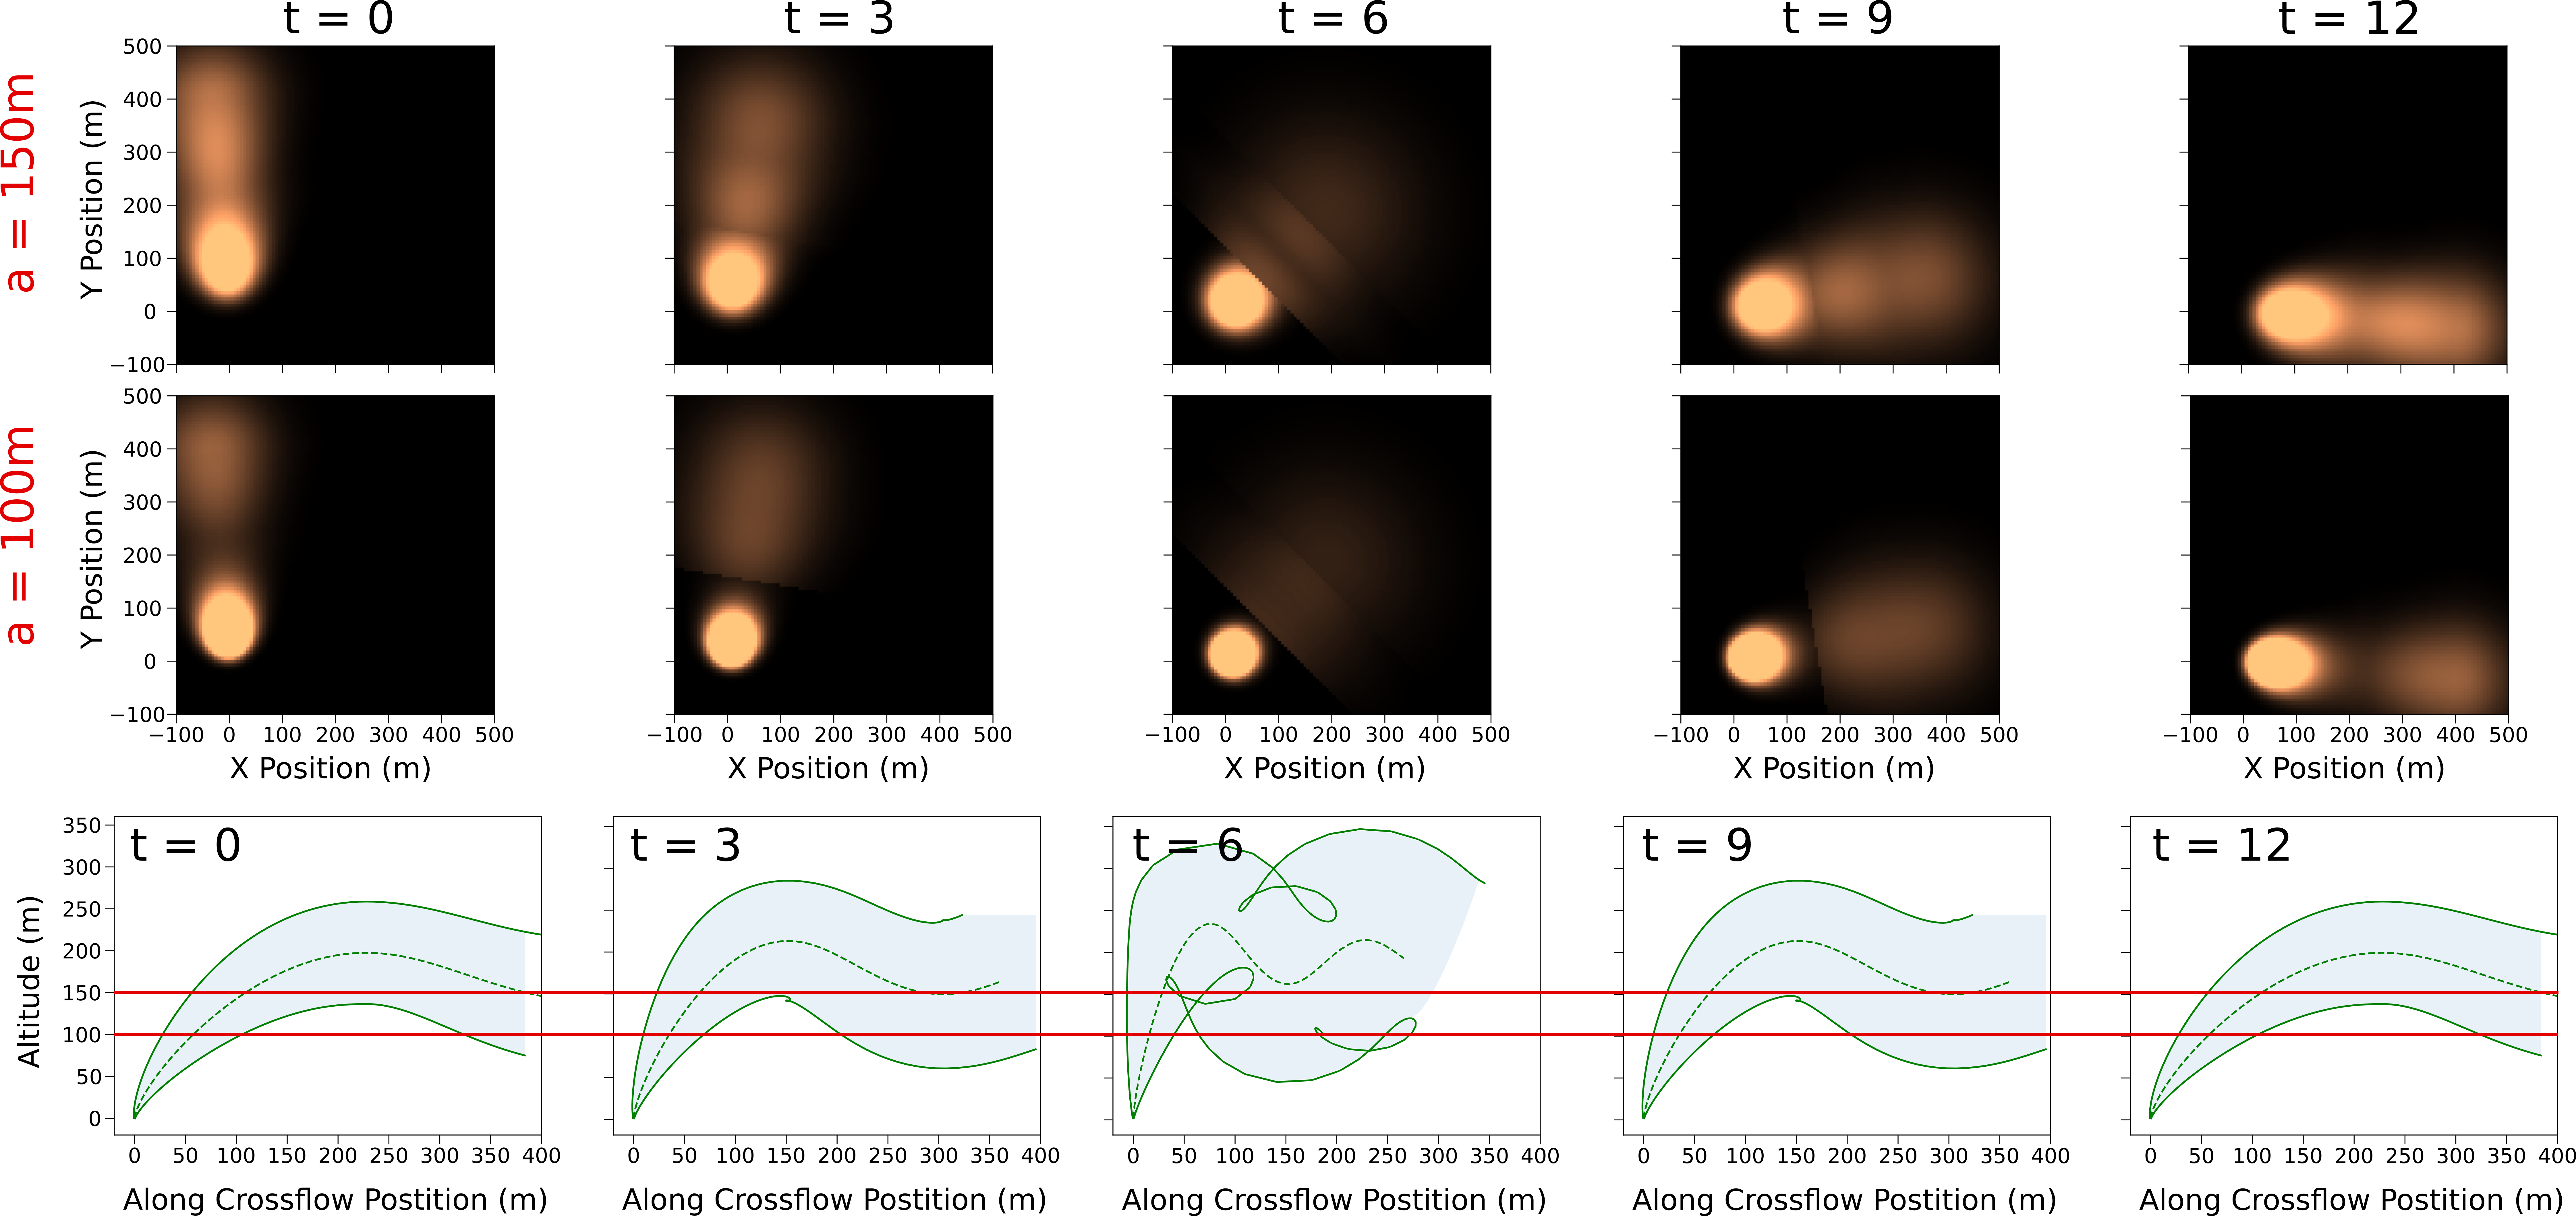
\includegraphics[width=1\columnwidth]{figures/sim_env.png}
    \caption{\textbf{Simulated field trial environment.} Generated environment for simulation trials at different snapshots for altitudes of \SI{100}{\meter} and \SI{150}{\meter}. As the current magnitude and heading changes, the plume expression changes shape and location over 12 hours. Plume intensity is shown in orange in the top plots. The bottom plots show a vertical cross-section of the plume envelope, along the crossflow direction, at different points in the tidal cycle, with the \SI{100}{\meter} and \SI{150}{\meter} horizontal planes marked.}
    \label{fig:sim_env}
\end{figure}

In these experiments, the \PHUMES model must estimate the vent area, vent fluid velocity, and both mixing coefficients from plume observation in the water column, starting with uninformative priors over each of these targets. A noisy current magnitude and heading function is provided to \PHUMES for use in the forecasting and updating step, as would typically be available from, for example, an auxiliary tiltmeter sensor (\cref{sec:aux_sensors}). For the \PHUMES update, 150 samples from an MH-MCMC chain are used to approximate the posterior distributions over the inference targets (this excludes an initial 50 samples of burn-in). In the first simulated dive, the robot executes a base-case uniformed lawnmower trajectory, placed to intersect the sweeping movement of the current. This trajectory is \SI{15}{\meter} in resolution, and covers a \SI{500}{\meter} by \SI{500}{\meter} area, with no rotation. For the second and third dives, trajectories are optimized using \PHORTEX for the 12-hour mission and consist of four, 3-hour long chained lawnmowers. Each lawnmower in the chain has a fixed resolution of \SI{10}{\meter}, and the height, width, origin, and orientation of each lawnmower are optimized to collect the most reward based on a plume forecast using the maximum \emph{a posteriori} (MAP) sample returned by the \PHUMES model for the four inference targets. The robot travels at approximately \SI{0.5}{\meter\per\second}, collecting binary observations every meter that is traveled. 

% Quality for this task is defined as collecting a high-proportion of in-plume samples over the course of a dive, revisiting a plume over the course of a dive, and collecting in-plume samples as far from the vent as the robot drives. 
\subsection{Simulation Experiments: Results}
\cref{fig:sim_traj_example} shows example planned trajectories and \cref{fig:sim_traj_perform} shows the distribution of each of the metrics of interest presented in \cref{sec:eval_metrics}---proportion in plume, spatial utilization, temporal utilization---for the three dives at each altitude tested in the trials. These results demonstrate that the \PHORTEX optimized trajectories significantly outperform the naive baseline, collecting over twice the proportion of samples in-plume, at least doubling the number of hours that the robot spends in a plume, and improving spatial utilization to nearly 100\% from 60-70\%. 

\begin{figure}[h!]
    \centering
    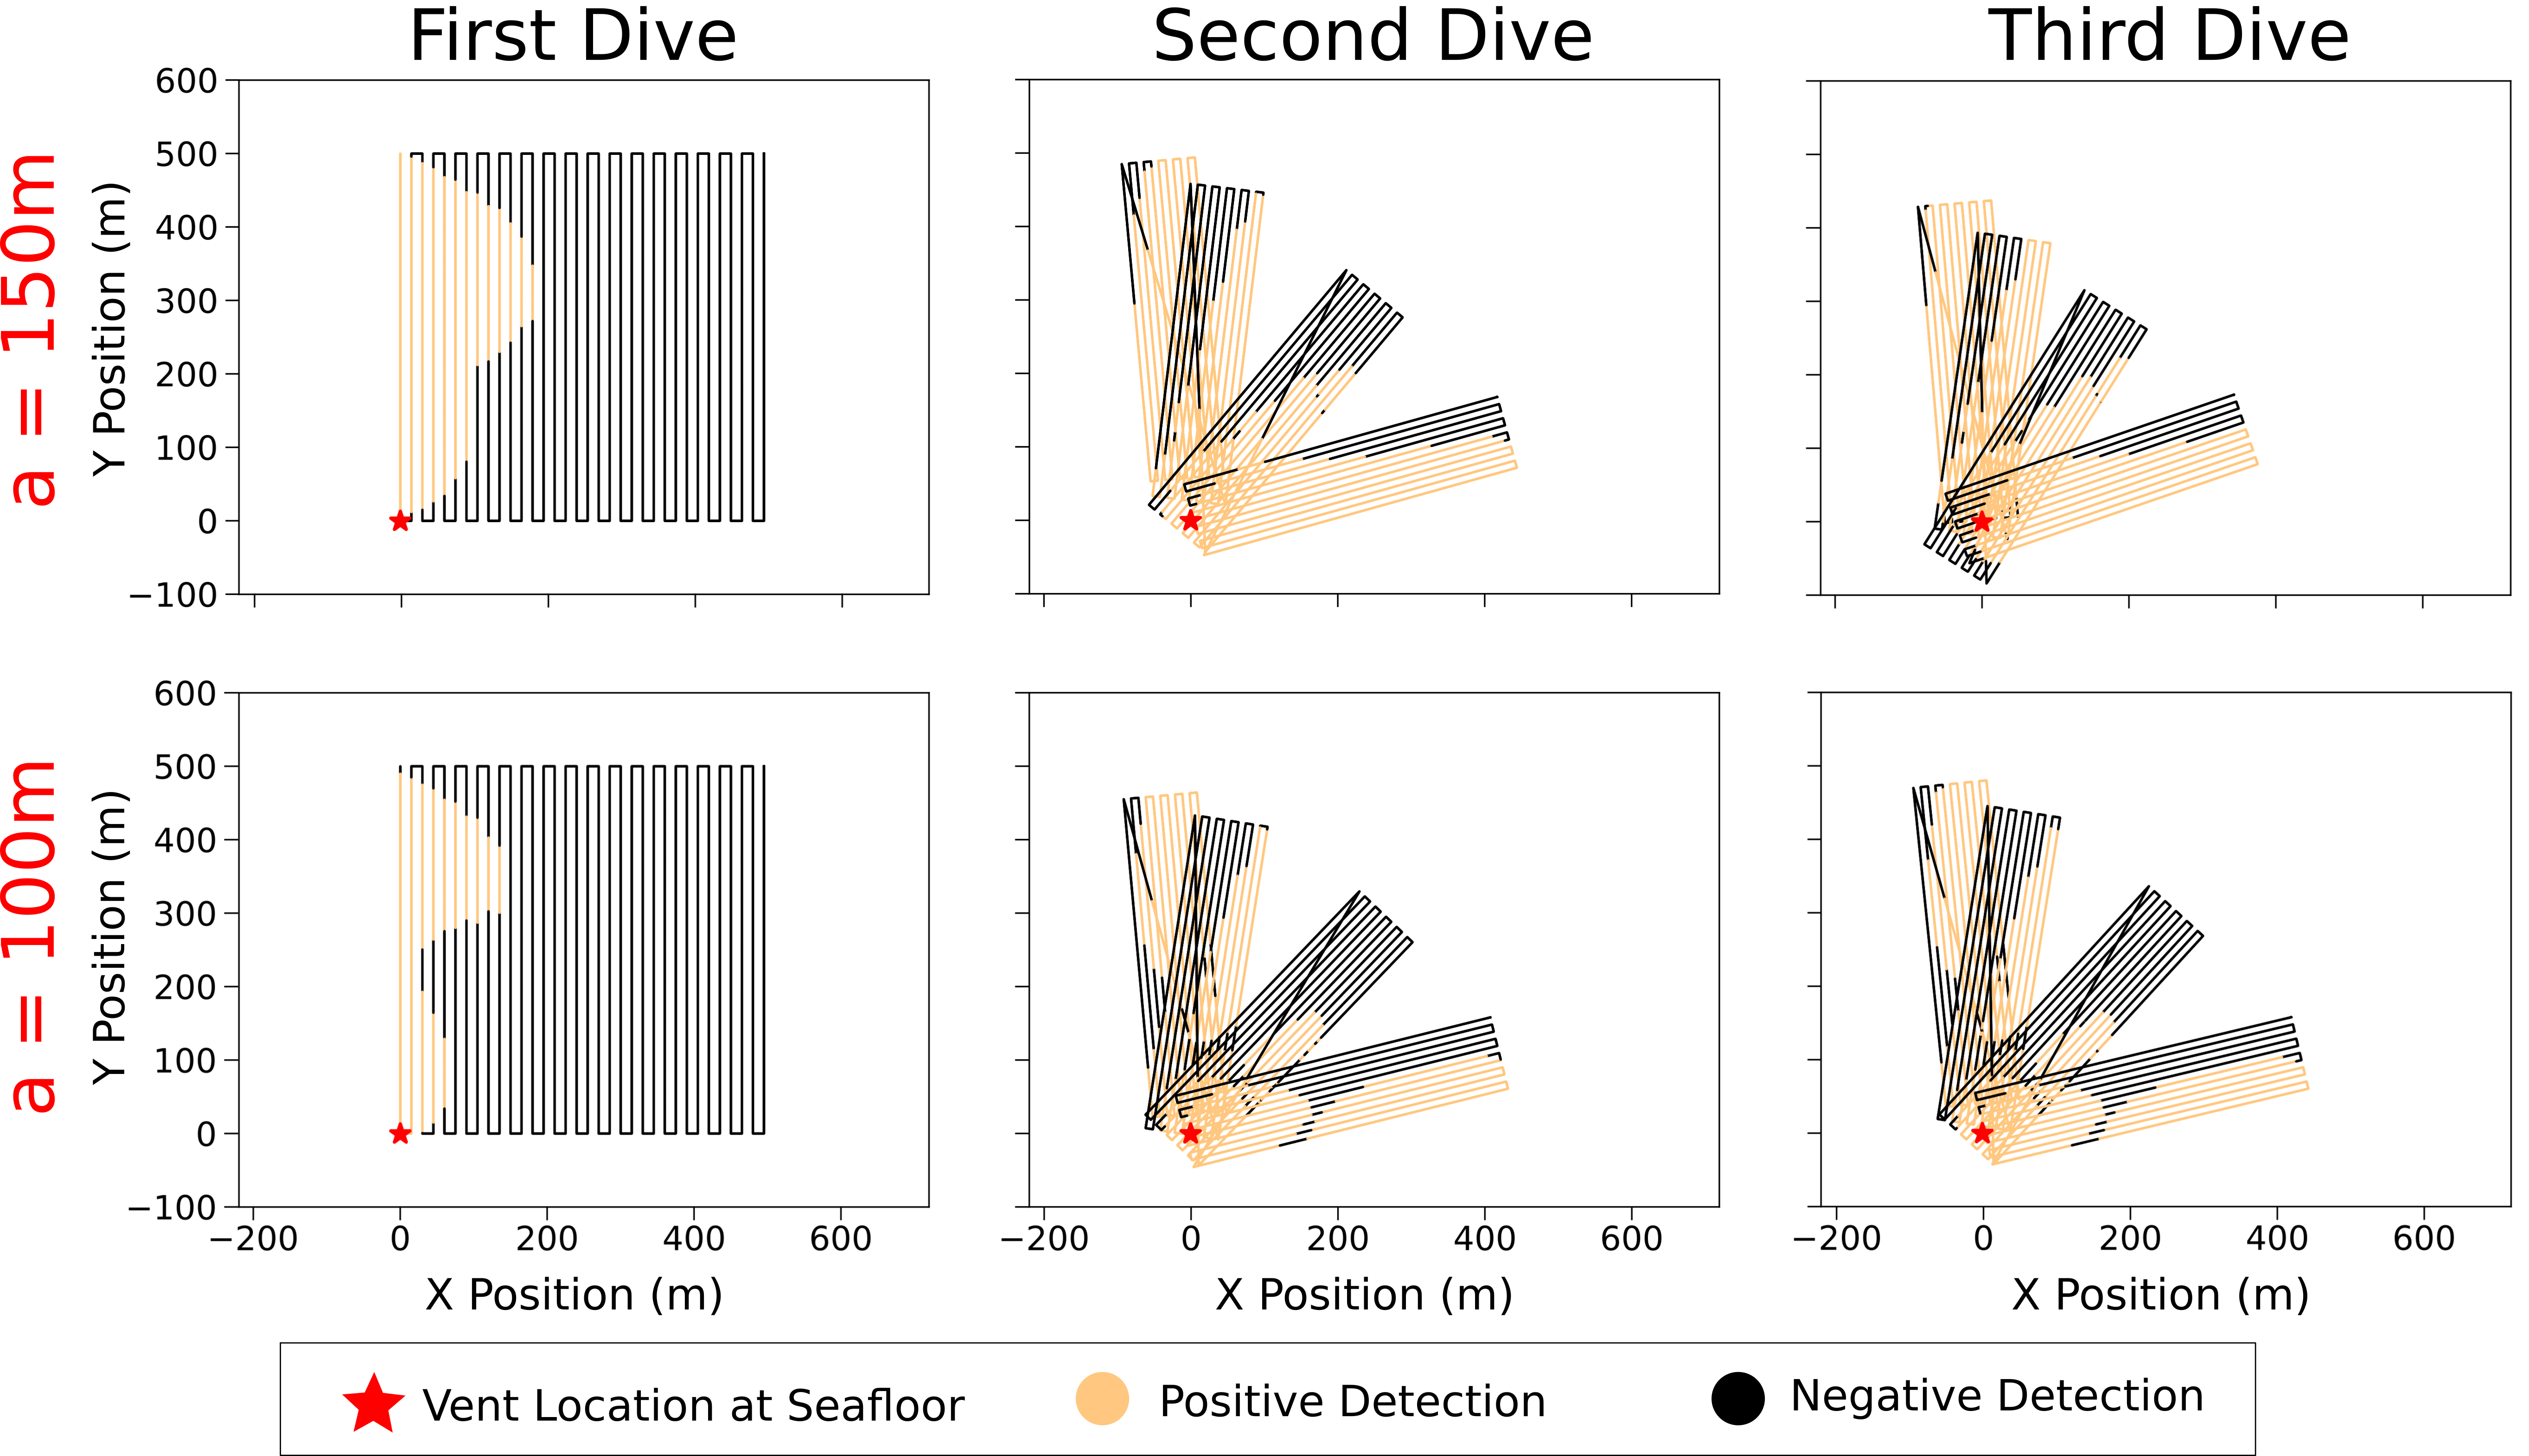
\includegraphics[width=0.85\columnwidth]{figures/sim_traj.png}
    \caption{\textbf{Naive and \PHORTEX-designed trajectories.} Trajectory examples for altitudes of \SI{100}{\meter} and \SI{150}{\meter}. The first dive is always a naive lawnmower; the second and third dive are \PHORTEX designed trajectories. \PHUMES is incrementally trained after each dive on the binary plume detections shown in this plot, which are sampled every meter traveled along the trajectory.}
    \label{fig:sim_traj_example}
\end{figure}

\begin{figure}[h!]
    \centering
    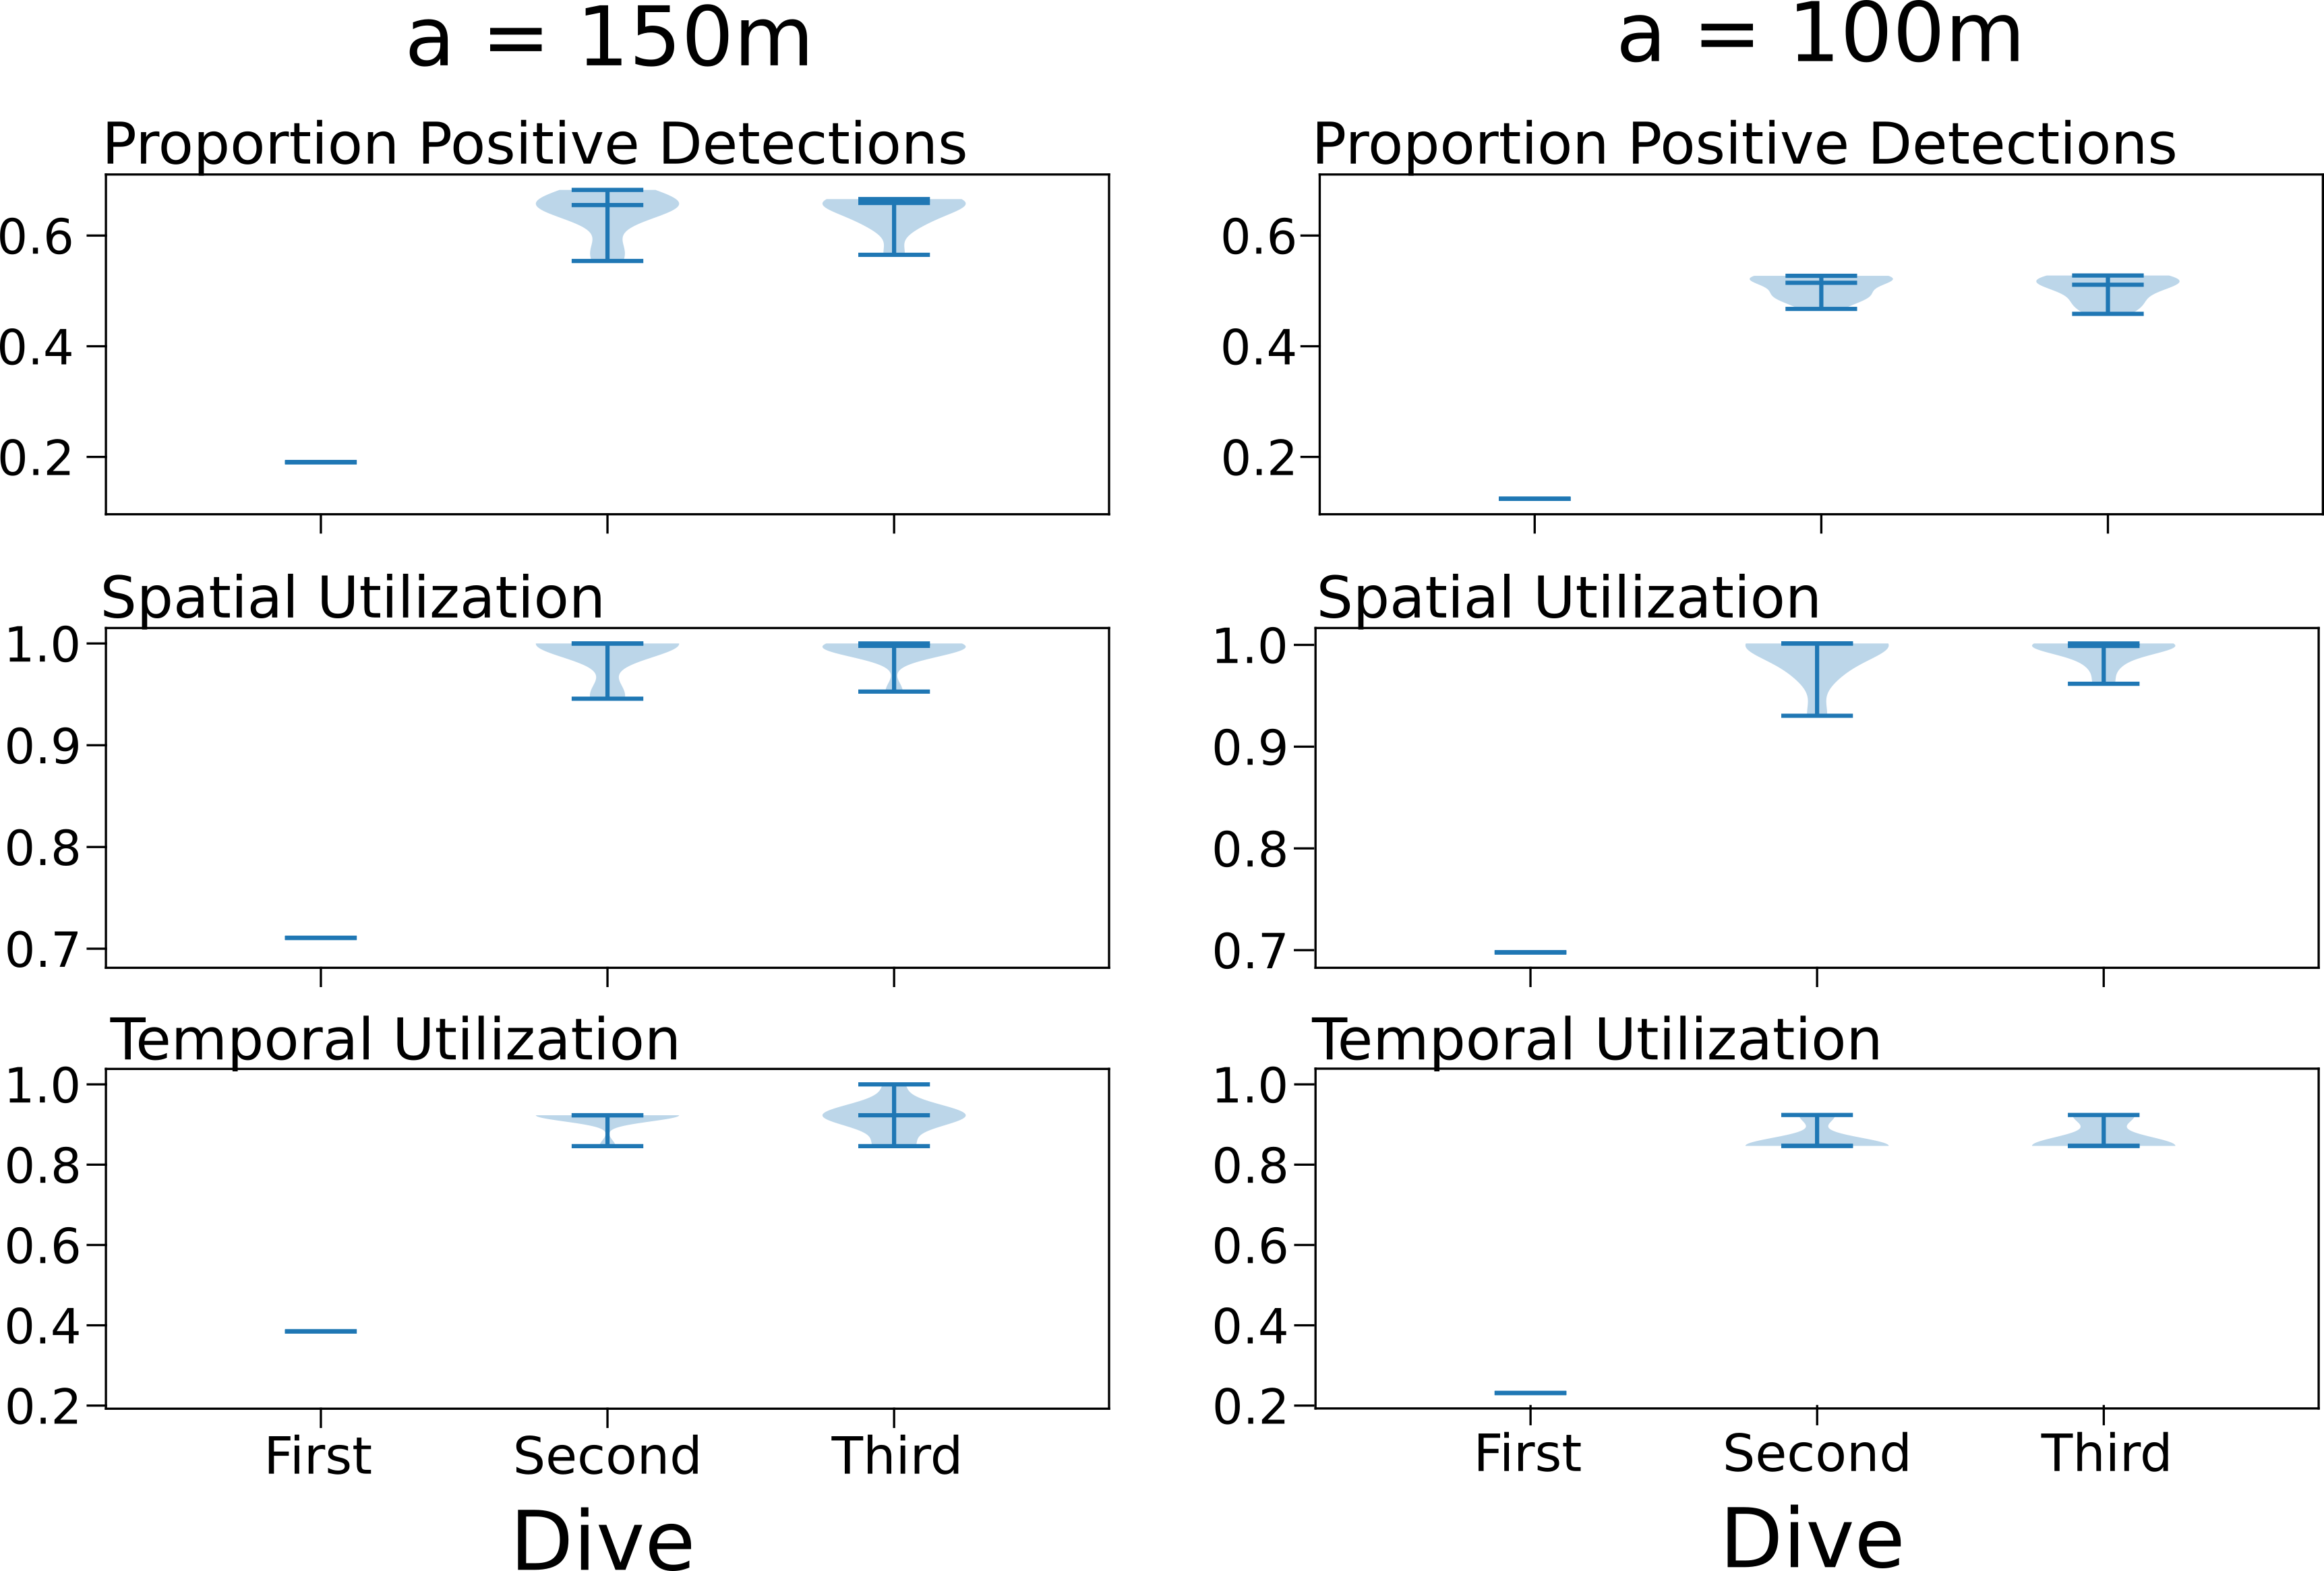
\includegraphics[width=0.75\columnwidth]{figures/sim_traj_performance.png}
    \caption{\textbf{Evaluation of the \PHORTEX trajectories.} The three-dive sequence, consisting of a naive lawnmower followed by two rounds of \PHUMES model training and \PHORTEX trajectory optimization, are evaluated for proportion of positive plume detections, spatial utilization, and temporal utilization (\cref{sec:eval_metrics}). The \PHORTEX-designed dives show a clear improvement in all three metrics, gathering more spatially and temporally diverse observations of the dynamic hydrothermal plume. Iterative rounds of \PHORTEX model-training and trajectory optimization continue to collect a high proportion of scientifically valuable observations.}
    \label{fig:sim_traj_perform}
\end{figure}


\paragraph{\PHUMES Model Validation}
The performance of \PHORTEX stays consistently high in the second and third dives, suggesting that \PHUMES quickly learns a sufficient model for planning from the small number of samples collected by the naive trajectories. To further understand the model learned by \PHUMES, we first qualitatively inspect the models learned by \PHUMES in two exemplar trials with data collected at \SI{100}{\meter} and \SI{150}{\meter} altitude during the initial naive survey of the first dive, as presented in \cref{fig:sim_model}. In the naive survey, less than 20\% of all detections are positive detections, and all detections only occur in the first 3 hours of the 12 hour mission. At an altitude of \SI{100}{\meter}, the robot essentially ``skims'' the bottom of the neutrally-buoyant plume; at \SI{150}{\meter}, the robot is consistently within the range of the neutrally-buoyant plume. Despite these altitude differences models learned in this example show remarkably similar characteristics---a predicted centerline no more than \SI{25}{\meter} off from the true environment's centerline, and a width that nearly completely envelopes the true plume distribution, which is promising for the context of planning missions. This is in contrast with an illustrative sample from the uninformative prior, which can arbitrarily produce plume structures that are significantly different in form from the true generating environment. It is also worth noting that despite training data only being available for 3 hours of the 12 hour simulated dive, the predictive quality of the model learned forecasts to an unseen time (t=9hrs) remains high. This largely demonstrates the advantage of using an embedded dynamics model in order to generate predictions of the state space to unseen times.

\begin{figure}[h!]
    \centering
    \includegraphics[width=\columnwidth]{figures/sim_mod.png}
    \caption{\textbf{Illustration of model learning.} Snapshots of the true generating environment are compared with an arbitrary sample from the prior distribution over \PHUMES parameters and the learned models from data collected by naive lawnmowers in both \SI{100}{\meter} and \SI{150}{\meter} simulation trials. In these two exemplar experiments, model learning performance is comparable between the \PHUMES models trained on data from different altitudes. The learned model, in comparison to the baseline sample, demonstrates a lower neutrally buoyant stem height, and is wider, and better explaining the data collected at the two sampling heights. Snapshots at different times show that the learned parameters robustly predict future shapes of the plume, even when trained on partial data available from the naive lawnmowers.}
    \label{fig:sim_model}
\end{figure}

To the quantify performance of the plume forecast generated by the MAP parameter sample after each trial, we compute the intersection over area (IoA) and intersection over union (IoU) between the true environment and each of the learned models after the naive and first \PHORTEX designed dives (\cref{fig:sim_phumes_perform}). A set of 10 parameter samples from the uninformative priors over the inference targets are used to generate an initialization performance distribution to show the breadth of forecast quality before any training. IoA (or recall) provides a number from 0-1 that expresses how many samples in the learned model are shared with the true generating environment. This number does not penalize false positives in the model: a value of 1 implies that all points in the model are contained by the environment, and a 0 implies that there are no points contained in the true environment. IoU (or precision) also provides a number from 0-1 that now penalizes false positives: a value of 1 implies perfect alignment between the model and environment, and a 0 implies no alignment. The comparison of these numbers helps to contextualize the performance of model learning. 

In \cref{fig:sim_phumes_perform}, we see that the learned models have a narrower performance window than the baseline samples, and that they generally exhibit very high IoA (up to 1), and a higher IoU (up to 0.9) than the baseline models (up to 0.75). With a high IoA, we can be confident that the learned models are placing value in areas for which there is plume, and with a higher IoU, we can be confident that the structure of the predicted regions with high value align well with the true environment. Taken together, a very high IoA with medium to high IoU suggest that trajectories planned with the \PHORTEX-trained models are very likely to plan for and successfully execute intersections with the targeted plumes, which is advantageous for our scientific task. We do not see a degradation of performance with different observations available between dives, suggesting that from very little data (a single naive dive), we can train an immediately useful model. Additionally, we note that there is a distinct difference in the distribution shapes of IoA and IoU between the altitudes across these trials. In particular, training from samples at \SI{150}{\meter} appears to be more consistently highly performant (IoA mode is at or near 1; IoU distributions skew towards 0.8) than at the lower altitude, which has a more distributed performance characteristic (with IoA skewed just about 0.8, and IoU centered just above 0.6). This has interesting implications for choosing deployment altitudes in practical missions, within the constraints of robot abilities (for instance, AUV \Sentry cannot swim over a certain altitude and maintain good localization, thus constraining what parts of a plume may be accessible in field deployments). We leave as future work the finer scale characterization of informativeness of different plume regions for model recovery in scientific settings.


\begin{figure}[h!]
    \centering
    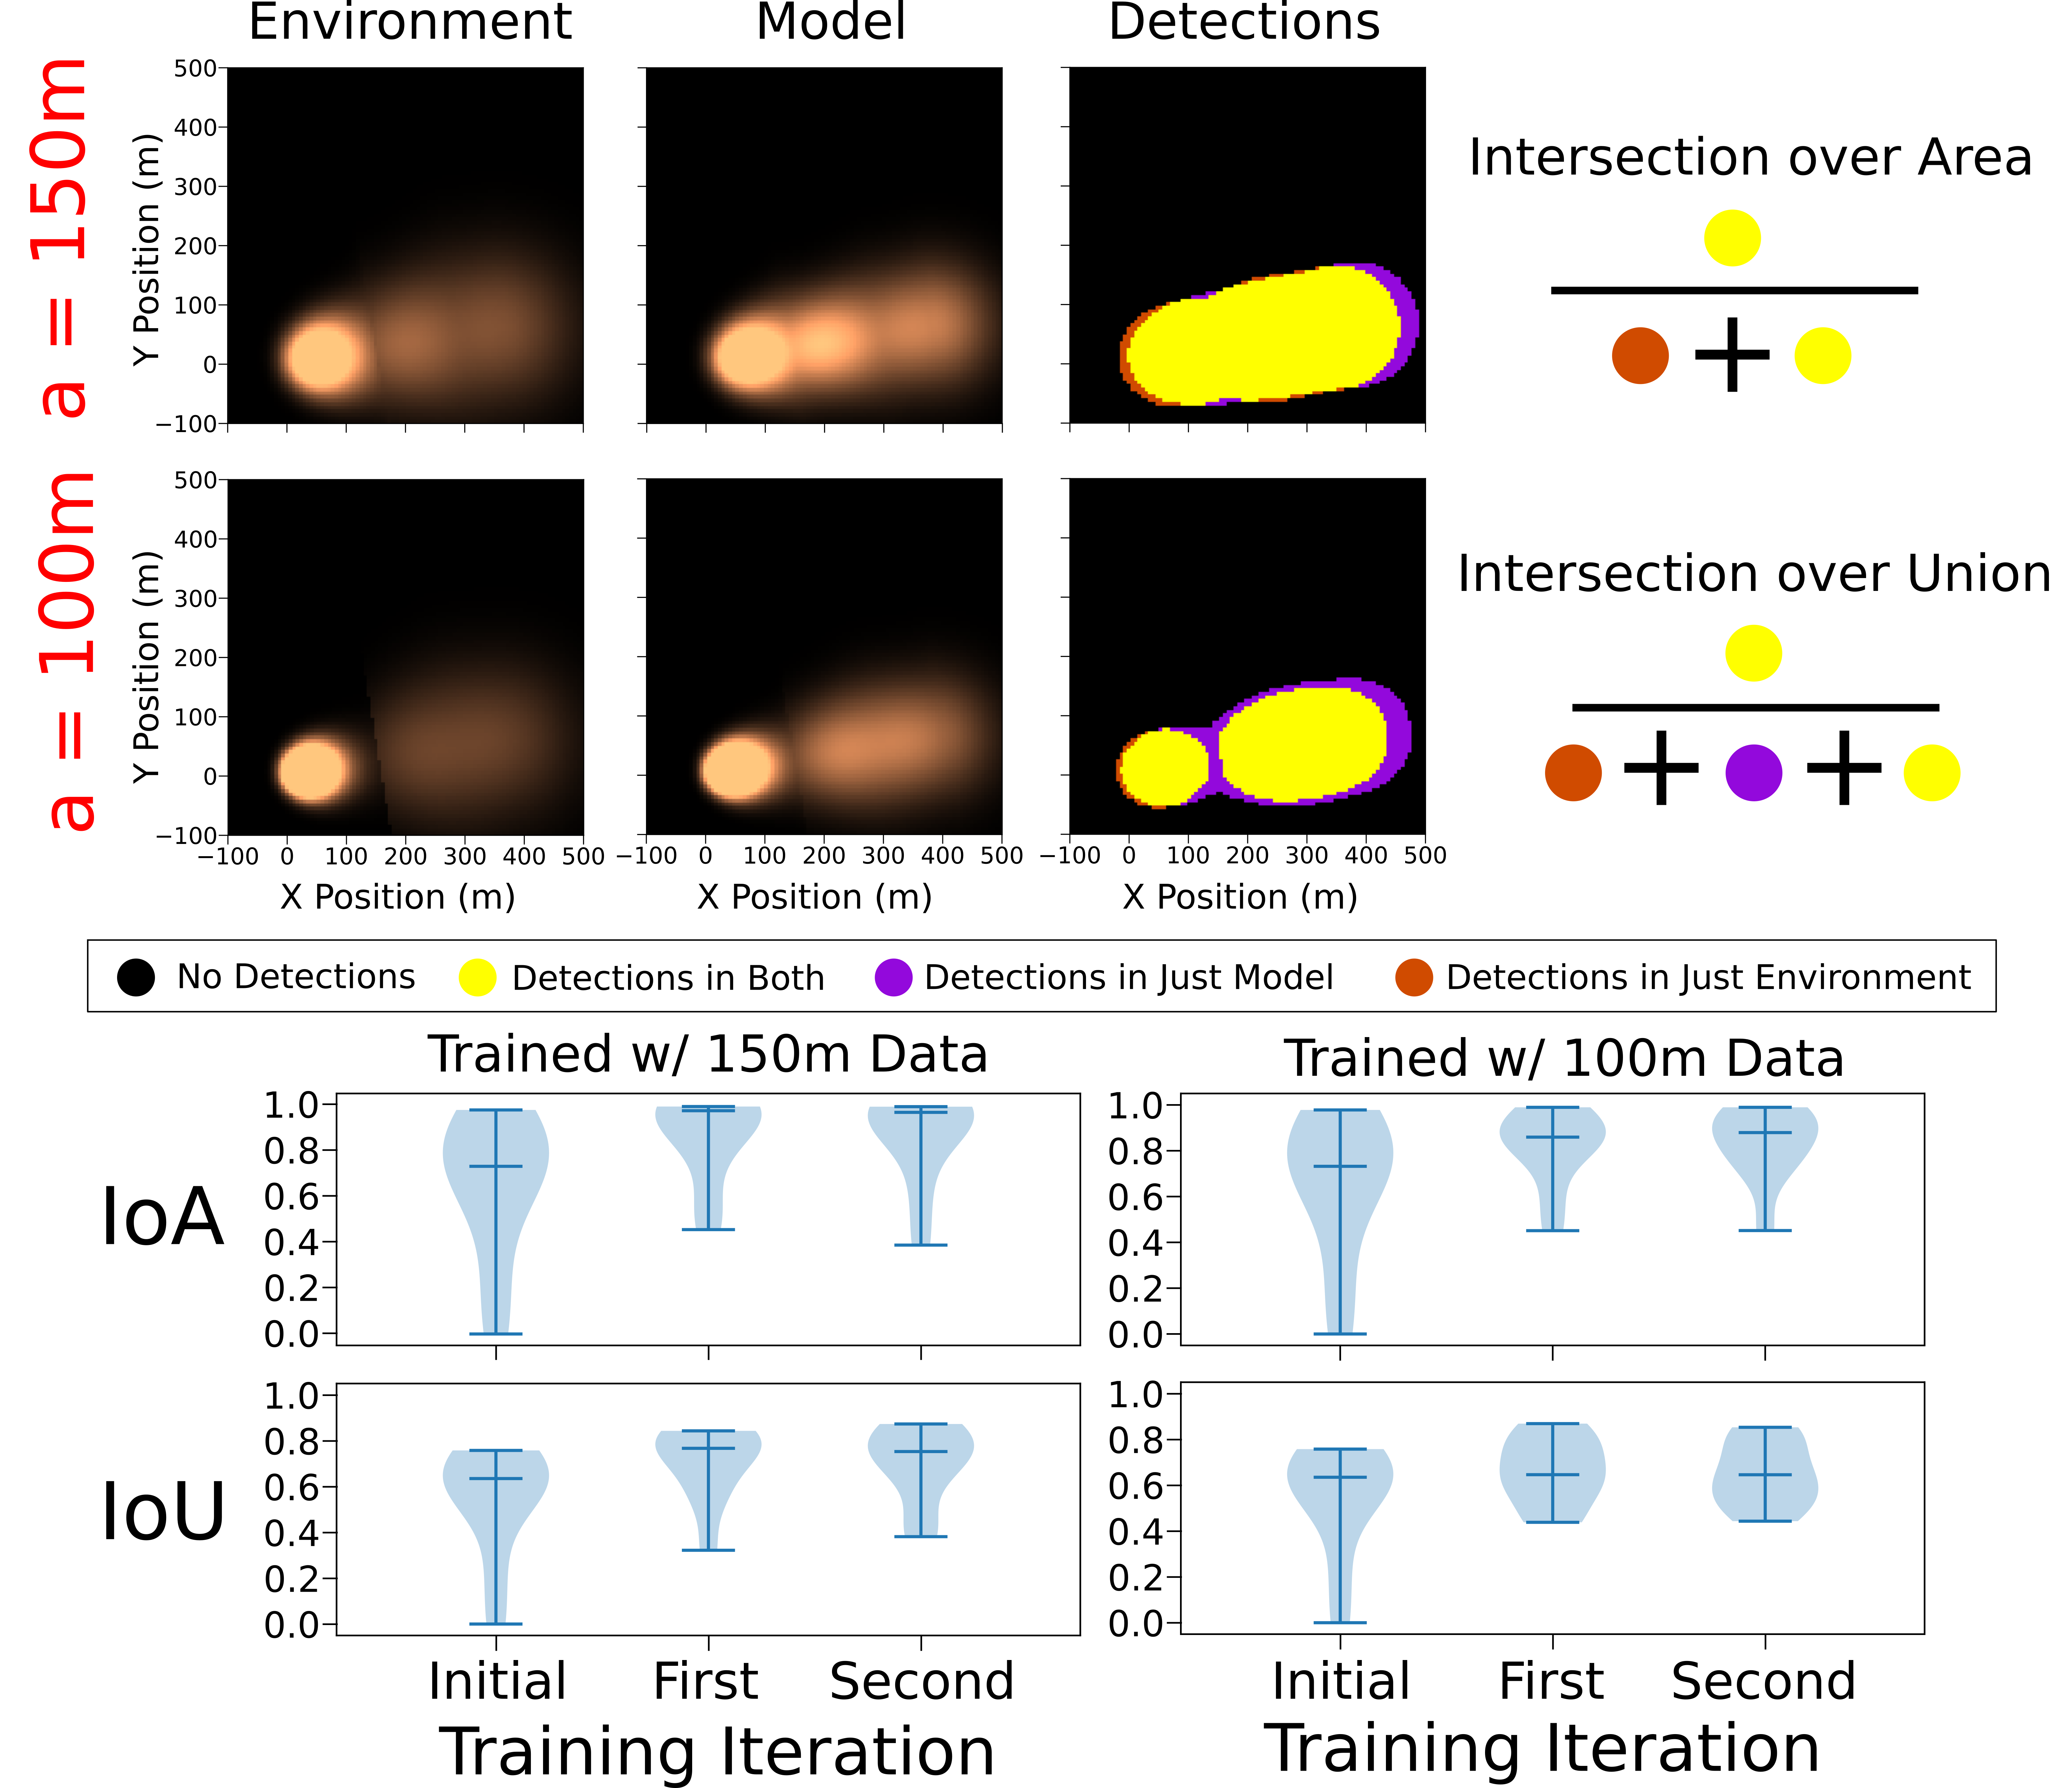
\includegraphics[width=0.9\columnwidth]{figures/sim_mod_performance.png}
    \caption{\textbf{Intersection over Area (IoA) and Intersection over Union (IoU) of trained models.} For each of trials trained from data at \SI{100}{\meter} and \SI{150}{\meter} altitudes, we compute the average IoA and IoU (using the method illustrated at the top) for a set of initial model samples (Initial), \PHUMES trained on the naive dive (First), and \PHUMES trained on the follow-up \PHORTEX-designed dive (Second). In general, we see the each of the iterative trained dives maintains similar performance; with high IoA and medium-to-high IoU that is consistently higher than initialized samples. Trials trained on data from \SI{150}{\meter} tend to have more performant model estimates (IoA near 1, IoU skewed above 0.8) compared to those trials trained on data from \SI{100}{\meter}.}
    \label{fig:sim_phumes_perform}
\end{figure}

% \begin{itemize}
%     \item We will first demonstrate \PHORTEX within the simulator we've created for generating plume funnels. We will show how \PHUMES converges to estimates of the true underlying distributions of initial conditions and parameter settings with and without noise. We will ideally show a graph that is RMSE of params versus mission iteration, and show a steep drop in error with steady improvement are iterations increase (fewer than 10 iterations will be graphed). 
%     \item We will additionally show performance on several key metrics, including reward versus iteration, total in-plume samples/accumulated reward under different model settings (e.g., number of samples in \PHUMES MCMC chain, prior uncertainty), and model mean and variance with each iteration. 
%     \item We will then show how sensitive trajectory optimization settings/chains are to collected reward, intending to show the advantage of using chains over a single highly-resolved lawnmower, at minimum.
%     \item If there is interest/time, we will then show how \PHORTEX performs in a numerically realistic simulator (as provided by our collaborator at University of Washington) and compute similar statistics as those indicated above. This addition would be used to demonstrate the complex real-time structure of plume snapshots, and show how the method generalizes to this setting. \VP{note that this is only if there is time; currently planning on only using the field results to demonstrate this, and may save simulation work for later tag-along conference/workshop paper}.
% \end{itemize}


\subsection{Field Trials with \PHORTEX at Sea}
In November 2021, \PHORTEX was used to design trajectories for AUV \Sentry at the Northern Guaymas Basin in the Gulf of California. Four deployments of AUV \Sentry were available to study the hydrothermal site. These deployments represent a planning spectrum, from fully human-designed surveys to fully \PHORTEX designed. We label the four deployments as follows:
\begin{itemize}
    \item \textbf{Dive H-Multi}: human designed, multi-task survey. This was the first deployment of \Sentry and the survey was designed to both attempt to find plume fluids and to bathymetrically map the local basin area (the map of which would be used as part of the safety check protocol for future deployments). This dive is representative of a standard nested strategy, in which progressively more targeted (finer resolution) surveys are used to study areas of interest. The dive was designed by a human expert who only had access to the approximate location of the target vent. The deployment lasted 21.3 hrs and collected 76,604 observations total.
    \item \textbf{Dive H-Plume}: human designed, plume-charting survey. This was the second deployment of \Sentry and the survey was hand-designed by the science party onboard the vessel to find and sample plume fluids. The science party had access to the performance of \Sentry in Dive H-Multi. The strategy was to sweep the basin above areas with known hydrothermal vents, and fly out into the basin in the direction that the plume fluids would be expected to advect. The deployment lasted 21 hrs and collected 75,430 observations total.
    \item \textbf{Dive HP-Plume}: hybrid human and \PHORTEX plume-charting survey. This was the third deployment of \Sentry and the survey consisted of trajectories designed by \PHORTEX trained by observations collected only in Dive H-Multi. Two of the trajectory primitives designed by \PHORTEX were replaced by ``naive'' lawnmowers placed over the known vent at two different times in the deployment. The deployment lasted 22.2 hrs and collected 79,792 observations total. Of these, 8.2 hrs and 29,438 observations were collected via the naive strategy.
    \item \textbf{Dive P-Plume}: \PHORTEX plume-charting survey. This was the fourth and last deployment of \Sentry. The survey was fully designed by \PHORTEX using observations only from Dive H-Multi, several days prior to this dive. The deployment lasted 9.9 hrs and collected 35,755 observations total. This deployment is notably much shorter than the other deployments due to increasing time constraints as the expedition was coming to a close. This deployment also used \Sentry in a ``depth-hold'' mode: whereas in all other dives \Sentry's depth followed the basin terrain, in this experiment the robot held an absolute depth.
\end{itemize}

\subsection{Field Trials with \PHORTEX at Sea: Results}
Using the metrics introduced in \cref{sec:eval_metrics}, we evaluate each of the four dives executed at sea to chart the space-time dynamics of a real hydrothermal plume as presented in \cref{tab:field_results} and visualized in \cref{fig:field_results}. Each dive took place at different times in the tidal cycle, on different days, and often at different altitudes in the water column, and thus the total plume samples available to collect during each dive is variable. With this in mind, we present and evaluate each dive quantitatively, and additionally qualitatively examine each as a case study for how different sampling paradigms perform in the real-world. There is no ground-truth available for the deep sea plume-charting problem; we evaluate each \Sentry dive assuming that the binary detections produced by the method in \cref{sec:sensor_models} are honest representations of the presence or absence of hydrothermally-derived fluids in the basin. 

The results of the field deployment in \cref{tab:field_results} demonstrate that \PHORTEX performs comparably to science expert-designed trajectories in the proportion of samples that are collected during dives, and importantly improves upon the spatial utilization (increasing both the range of the most distal plume detection and effectively utilizing of the entire explored range). This is most evident in the HP-Plume dive, in which the human designed portion is a naive lawnmower placed ``on top'' of the vent; the \PHORTEX-designed trajectory collects samples over twice as far from the plume source. Absolute temporal utilization is similar to human surveys; however the distribution of detections within the temporal utilization windows is improved --- for human surveys, detections tend to be ``bunched'' to either the first half (as in H-Plume) or second half (as in H-Multi). We see this most sharply in HP-Plume, in which 90\% of positive detections collected by the human-designed survey occurred only in the second of the two lawnmowers, from hours 20-23. In contrast, \PHORTEX designed trajectories collected detections more uniformly over the entire dive.  \cref{fig:field_results} shows the qualitative structure of each dive and showcases the diversity in the resulting datasets.

% Evaluating the efficacy of human- and \PHORTEX-designed trajectories in charting the space-time dynamics of a real-world hydrothermal plume is challenging. Unlike the simulation experiments, there is no ground-truth plume chart available and evaluating the counterfactual --- if \PHORTEX had gone here instead, how many more observations of the plume would have been collected? if we had used a naive planner instead of \PHORTEX for this deployment, how many fewer observations of the plumes would we have?--- is not straightforward. Due to operational constraints and the value of ship time, using an entire deployment of \Sentry to implement a lower-performing baseline is prohibitively wasteful; each deployment attempts to make the best use of available data to accomplish the task of plume charting.  In the remainder of the section, we evaluate each \Sentry dive using the metrics introduced in \cref{sec:eval_metrics}, assuming that the binary detections produced by the method in \cref{sec:sensor_models} are ground-truth detections and non-detections. 

% We look at several key metrics for each deployment: proportion of positive plume observations, utilization of spatial extent, and utilization of temporal dive window. The first metric, proportion of positive plume observations, is simply the number of observations collected in a dive that were classified as in-plume by the binary sensor model we describe in \cref{sec:sensor_models}. The second metric attempts to show how spatially effective the design of the survey was by first showing the absolute range that positive detections were made as a measure of distance from the chimney vent location and second showing how that range fit with the overall design of the survey. For example, if detections were made up to 300 m away from the vent, but the robot traveled up to 1 km away, then the survey spent too much time outside of the detectable plume region and would not be as effective as a survey that only traveled 200 m away but stayed well within the detectable plume range. Finally, the last metric is a measure of how effective the survey was at \emph{staying in} or \emph{revisiting} a plume over time. Given the duration of these missions, it is important to use the entire mission window for the task at hand; moreover temporally ``diverse'' observations are of scientific interest generally. We report the proportion of dive hours with at least 10\% or more positive detections.



\begin{table}[h!]
    \centering
    \begin{tabular}{c|c|c|c|c|c}
        Dive & Duration & Total Obs. & Prop. In-Plume & Spatial Util. & Temporal Util.  \\
        \hline
        H-Multi & 21.3 hrs & 76,604 & 22.3\% & \SI{300}{\meter} (19\%) & 9-17,20-21 (52\%) \\
        H-Plume & 21 hrs & 75,430 & 10.9\% & \SI{900}{\meter} (64\%) & 2,5-8,10-11,15-16 (43\%) \\
        \hline
        HP-Plume & 22.2 hrs & 79,792 & 41.8\% & \SI{600}{\meter} (100\%) & 1-3,5,7,11-23 (81\%) \\
        HP-Plume (H) & 8.2 hrs & 29,438 & 42.3\% & \SI{250}{\meter} (100\%) & 5,7,20-23 (75\%) \\
        HP-Plume (P) & 14 hrs & 50,354 & 41.5\% & \SI{600}{\meter} (100\%) &  1-3,11-20 (93\%)\\
        \hline
        P-Plume & 9.9 hrs & 35,755 & 12.8\% & \SI{450}{\meter} (100\%) & 1,5,8,9 (40\%)
    \end{tabular}
    \caption{\textbf{Per-dive statistics for field trials of \PHORTEX.} The spatial utilization is reported as both the most distal plume detection (measured from the plume origin) and the ratio of the most distal plume detection over the farthest distance that the robot traveled from the plume origin. Temporal utilization shows both which hours contain at least 10\% positive plume detection and what fraction of the total deployment duration contained such detections. The deployment HP-Plume is broken further into human designed (H) and \PHORTEX designed (P) portions for direct comparison.}
    \label{tab:field_results}
\end{table}

\begin{figure}[h!]
    \centering
    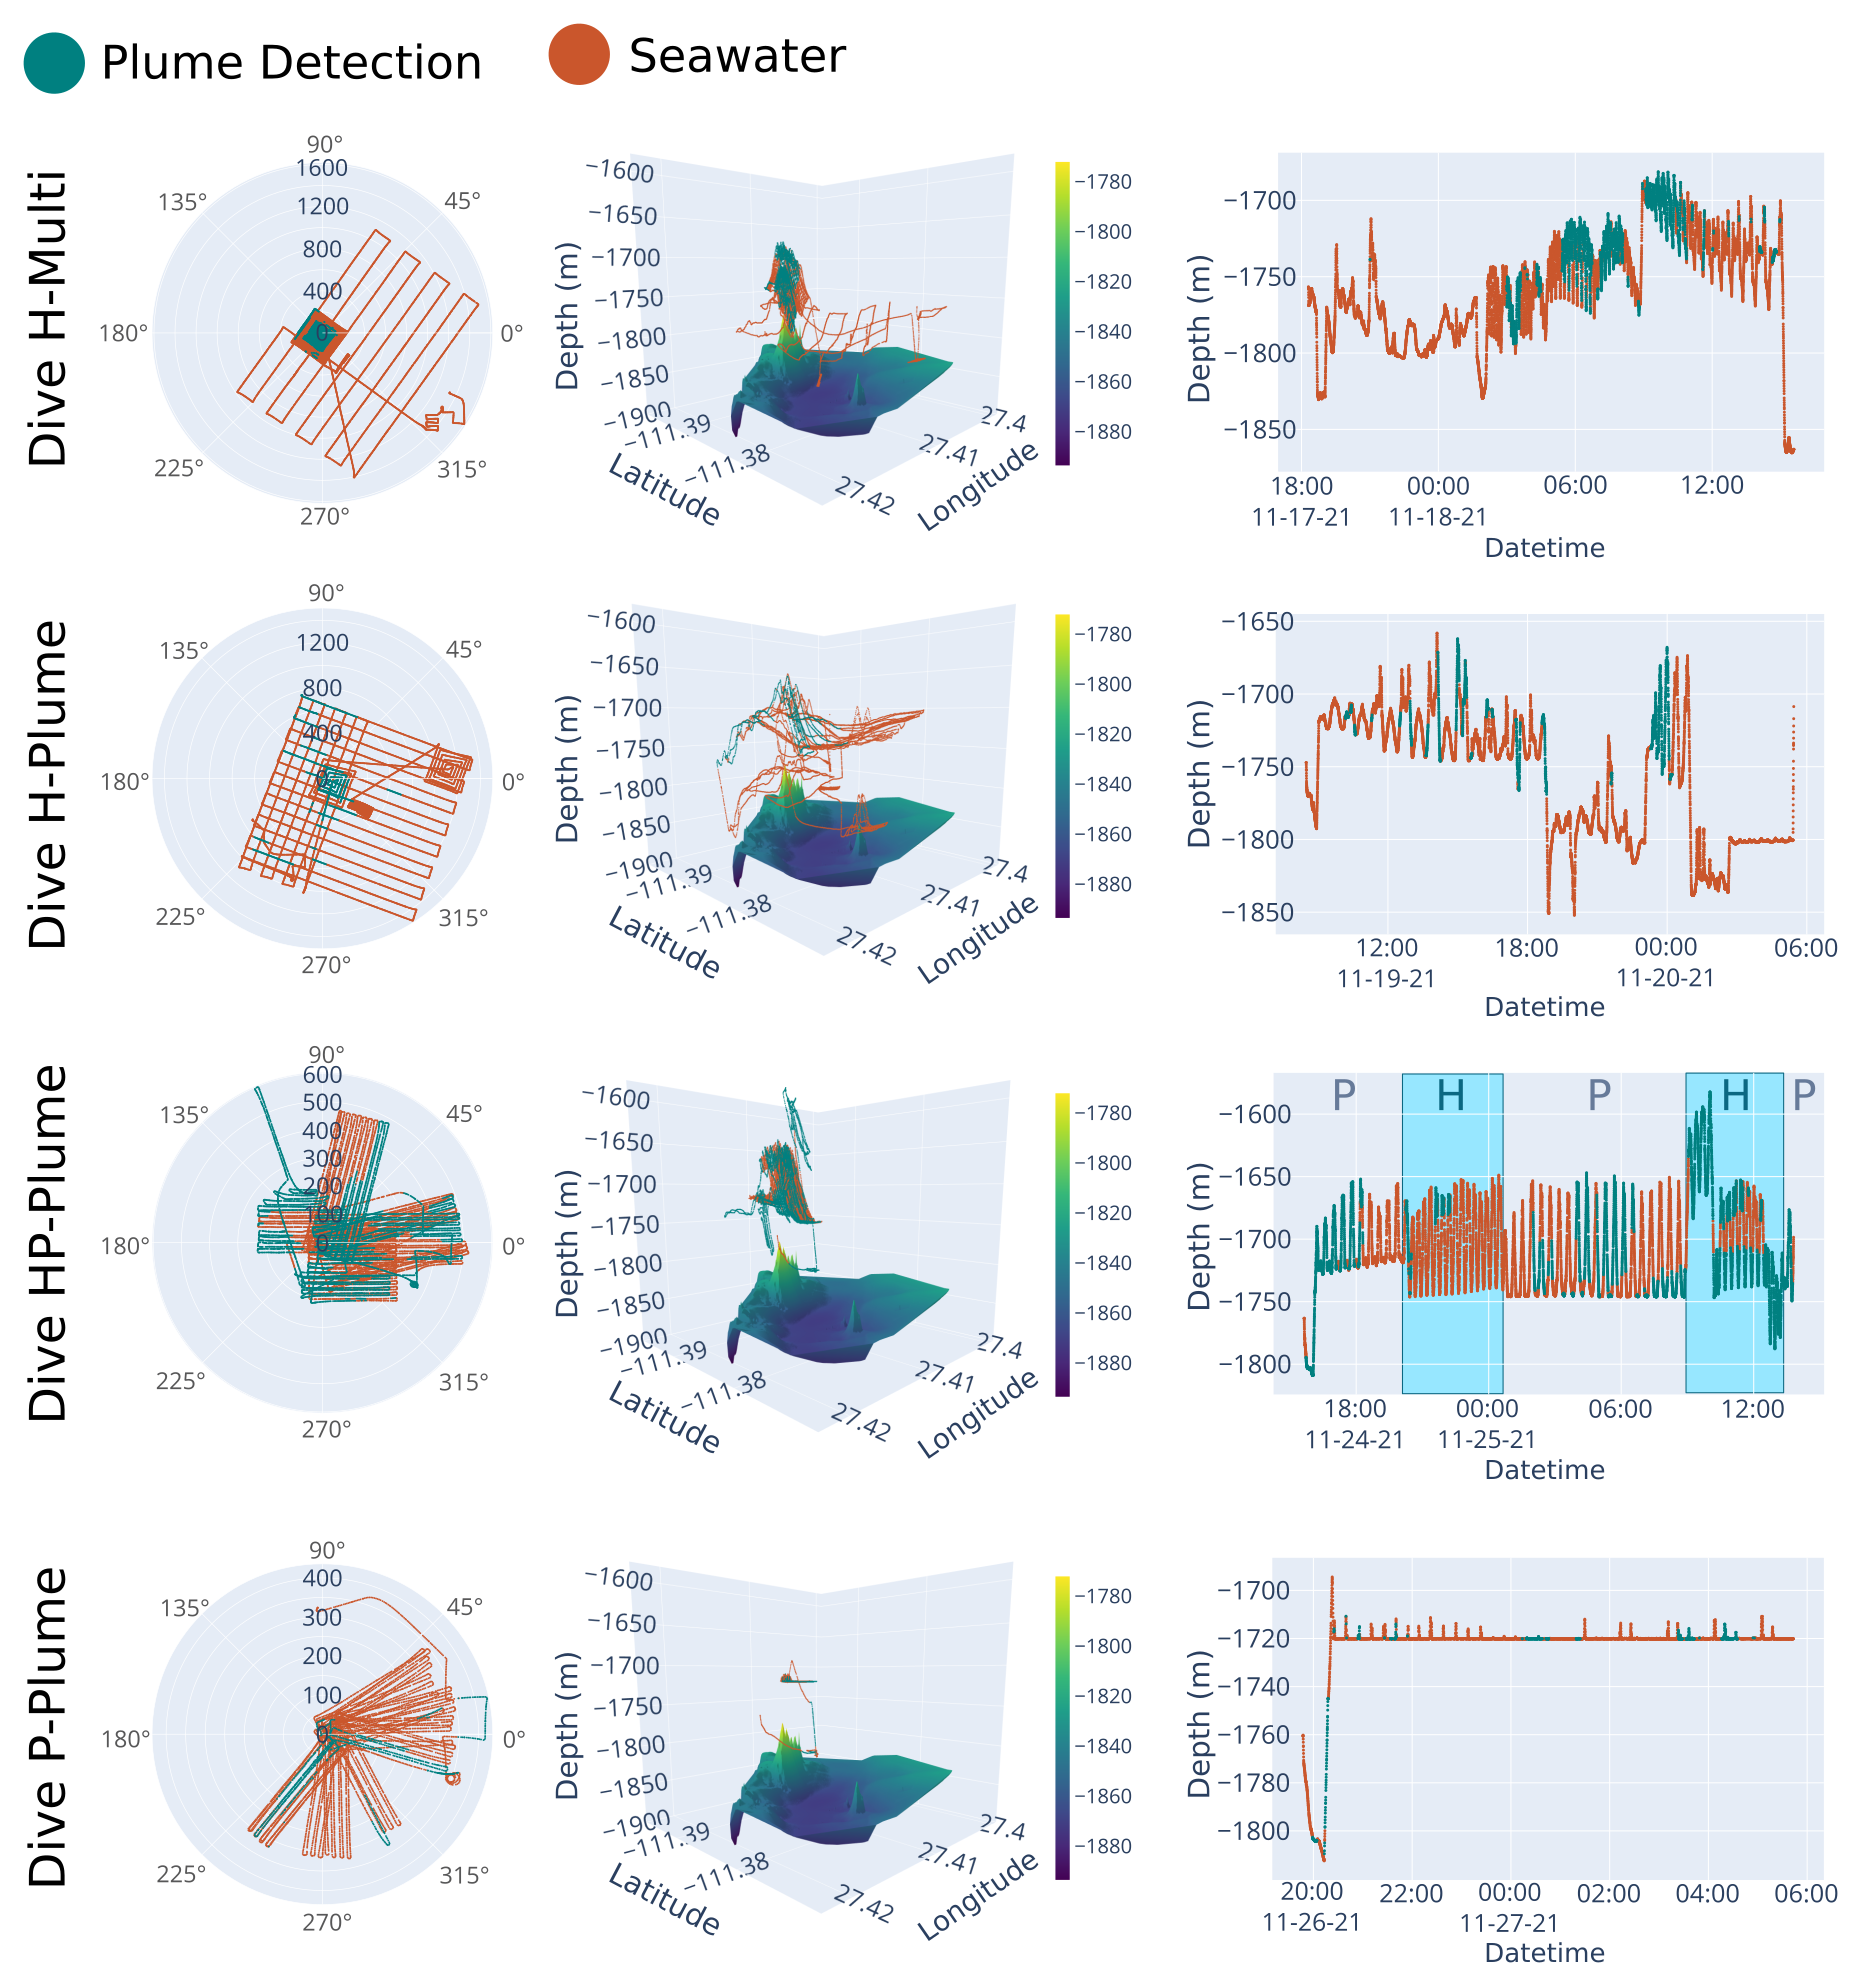
\includegraphics[width=1.0\columnwidth]{figures/detections_data.png}
    \caption{\textbf{The four field dives of AUV \Sentry.} All data is plotted according to its detection identity (in-plume or seawater). The first column shows a top-view of the dive trajectories in polar coordinates, in which angle and radius is computed relative to the chimney coordinate of the vent of study. In the center column, the 3D path of the vehicle over the rendered bathymetric terrain is provided. All but Dive P-Plume were dives conducted in altitude-hold mode with \Sentry, and so the trajectories show obvious changes in elevation; in contrast Dive P-Plume was held in depth-hold mode, so most observations are gathered within a depth-plane. The final column shows a time series versus depth of the detections collected. In Dive HP-Plume the portions of the dive that were human-designed and \PHORTEX-designed are labeled with H and P, respectively. As can be seen in the Dive HP-Plume time series, the two human-designed trajectories have significantly different performance, despite being in locally similar regions of the spatial domain. }
    \label{fig:field_results}
\end{figure}

In this field deployment, we demonstrate that \PHORTEX is a useful and practical tool for plume-charting. The performance of trajectories designed with \PHORTEX are comparable to those designed by human experts with key improvements in spatial and temporal utilization. It is further worth highlighting that \PHORTEX was trained only on data collected during the first dive, H-Multi, and reasonable performance during P-Plume using week-old training data emphasizes the long-range forecasting ability of the approach. Practically, the automated nature of \PHORTEX operationally alleviates significant decision-making burden on a science team and the trajectory-design burden on the \Sentry team; the ability to ingest data from external sensors and previous \Sentry missions, and produce trajectories that can be seamlessly ingested by the safety checking system without human intervention is of considerable benefit in the field. Moreover, the intermediate products of \PHORTEX, such as \PHUMES forecasts, are useful for other tasks in field operations, such as deploying other instruments or prioritizing instrument deployment order based on temporal changes in the environment by virtue of yielding rich context easily interpretable by the science team. 

% Similarly, \PHORTEX is trained on significantly less data than what the human experts had access to throughout the cruise; this emphasizes the advantage of the model-based, data-aggregation approach in \PHUMES. 

\paragraph{\PHUMES Validation with Basin Observations}
While there is no external ``ground-truth'' that we can use to evaluate the performance of \PHORTEX, we can compare the \PHUMES model trained on external and binary \Sentry observations with snapshots of the vertical distribution of turbidity near the hydrothermal ridge to get a sense for the utility of the \PHUMES model. After training, \PHUMES estimated the fluid exit velocity from the target chimney to be \SI{0.58}{\meter\per\second}, the vent area to be \SI{0.82}{\meter\squared}, and the vertical and horizontal mixing coefficients to be 0.15 and 0.19, respectively. Simulating these conditions with an initial vent temperature of \SI{340}{\celsius} and salinity of 34.908 PSU under a nominal crossflow of \SI{0.11}{\meter\per\second}, we compare the time-averaged plume height and width with the turbid intrusion that is observed in vertical casts of a shipboard rosette. The rosette was lowered and raised through the water column using a cable and winch on the ship; several vertical transects were collected over the course of the research cruise at the target autonomy site in addition to other sites throughout the basin. In \cref{fig:field_valid} we show two vertical transects, one conducted about \SI{100}{\meter} from a known vent, and one conducted \SI{600}{\meter} from the same vent. We see that within the model regions for predicted plume intrusions in the water column, strong turbid signals are observed in both vertical transects. This is indicative that the learned \PHUMES model is capable of uncovering the structure of the hydrothermal plume and lends confidence that the model is informative for planning sample trajectories that will intersect with plume fluids.

\begin{figure}[h!]
    \centering
    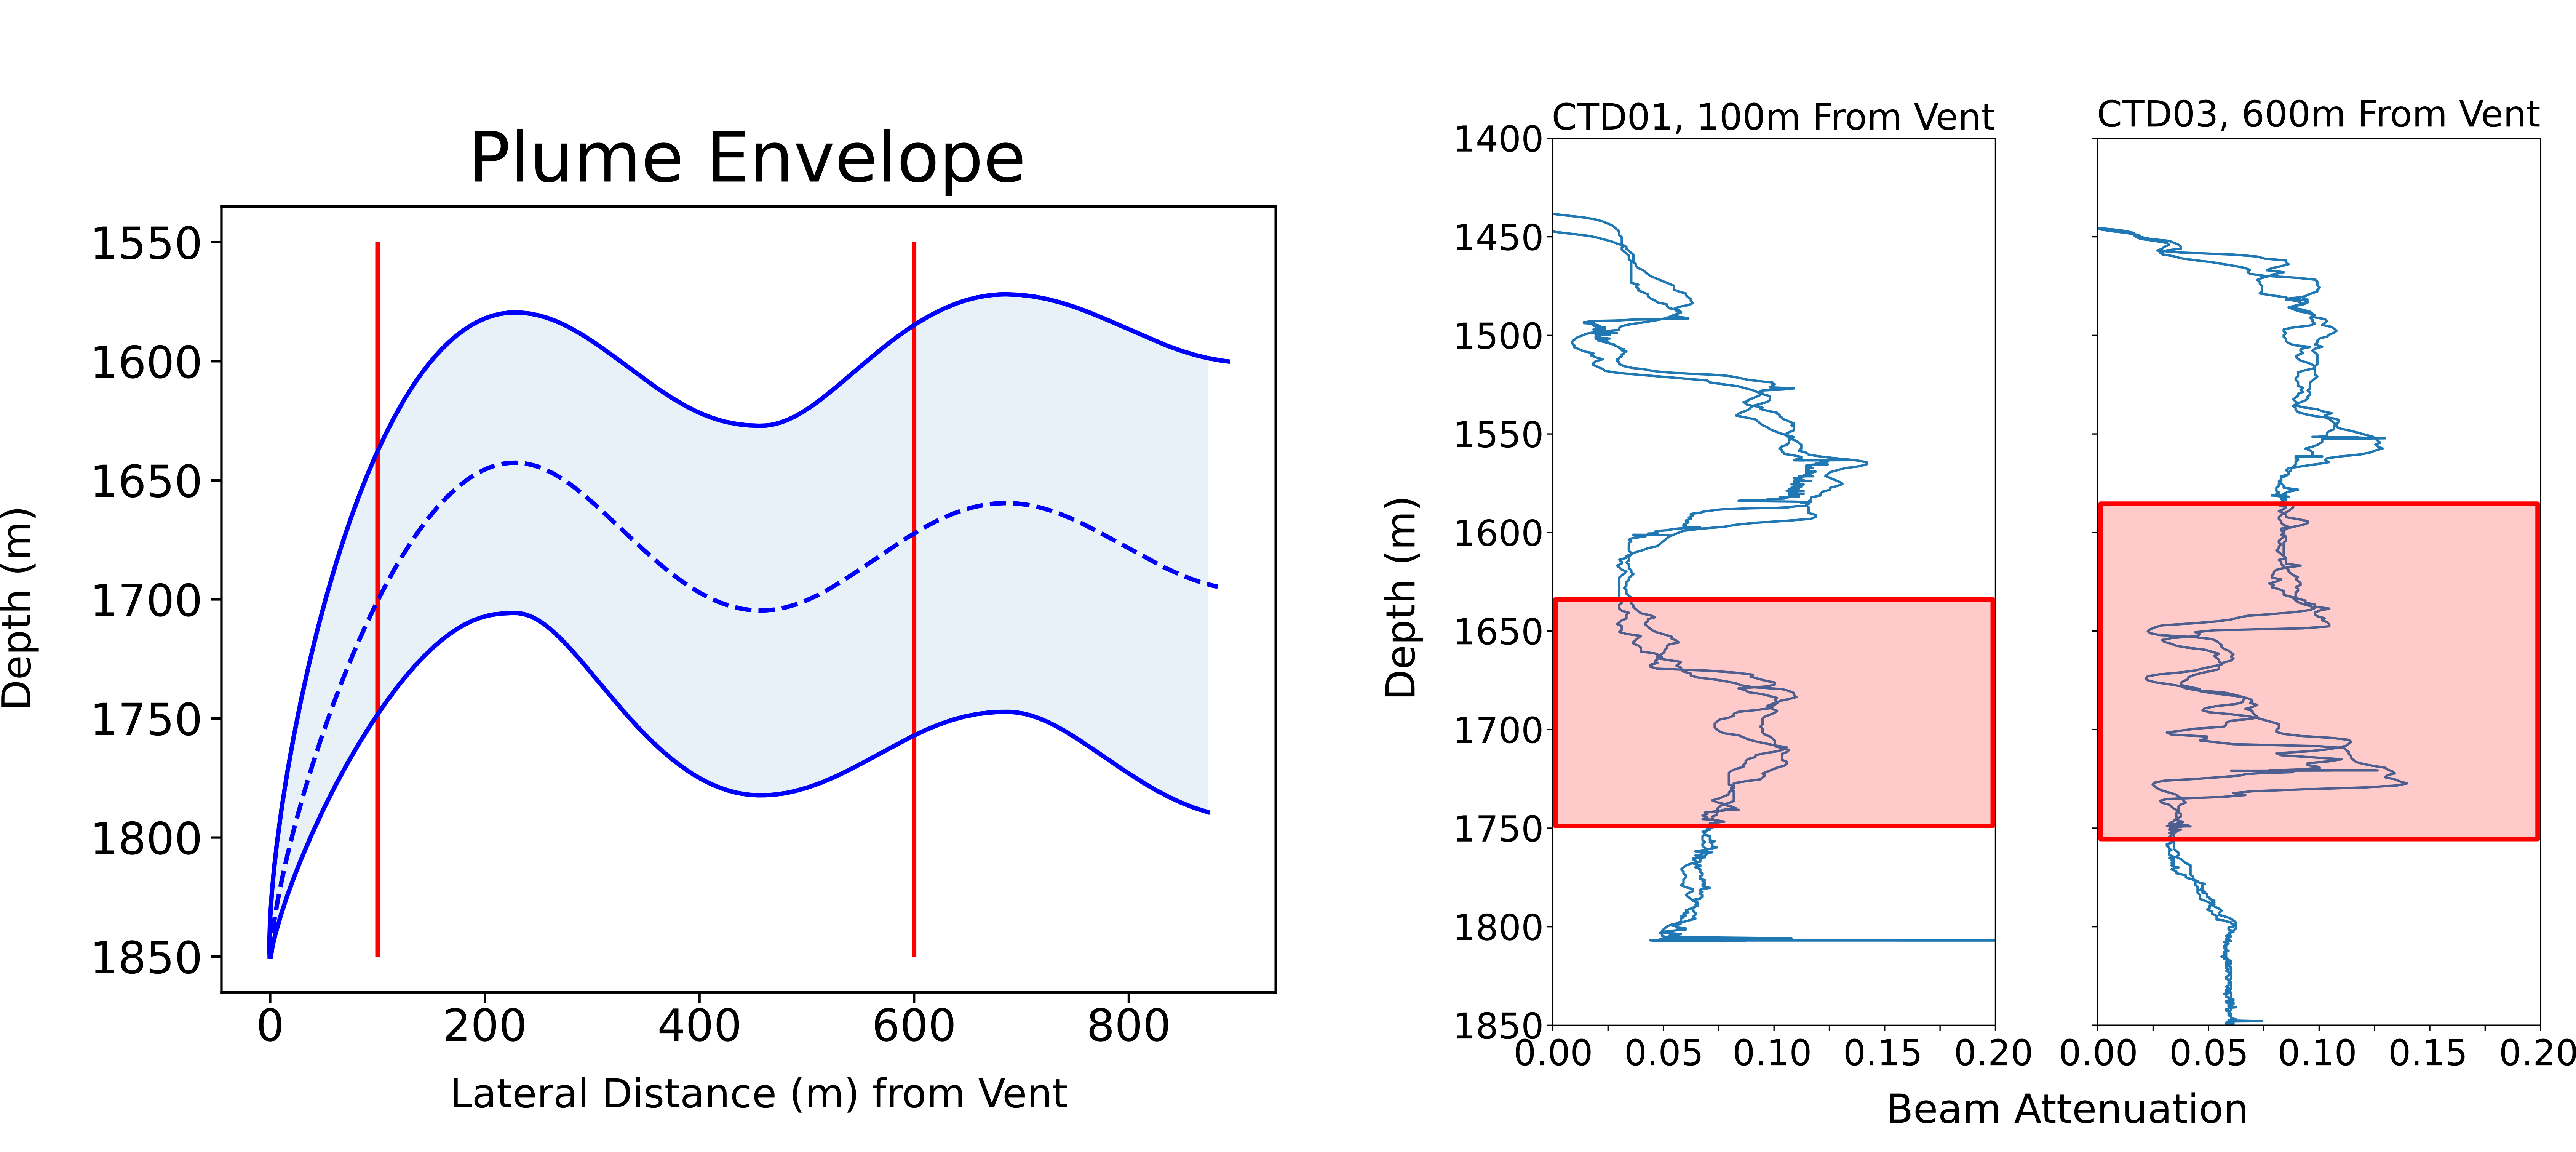
\includegraphics[width=1\columnwidth]{figures/field_validation.png}
    \caption{\textbf{Validation of \PHUMES model trained at sea.} We compare the nominal plume estimate from \PHUMES trained on at-sea data and \Sentry observations with vertical transects of turbidity from shipboard rosette. The plume envelope is the average plume estimated by \PHUMES for a nominal crossflow of \SI{0.12}{\meter\per\second}. Vertical red lines mark \SI{100}{\meter} and \SI{600}{\meter} laterally from the originating vent, for which vertical CTD casts were conducted. The region that the model estimates containing the lowest plume intrusion in the water column is highlighted on the turbidity transects. There is agreement between the model estimate and the transect data on the location of this turbid layer.} 
    \label{fig:field_valid}
\end{figure}


% \td{Note that this section is under construction! An overview of what this section will entail is below!}

% \begin{itemize}
%     \item This section will primarily present 4 trials that we performed while at sea -- 1 designed completely by hand, 2 partially designed by a person and by \PHORTEX, and one completely designed by \PHORTEX. The intent is to show the ``planning spectrum'' from fully-human to fully algorithmic, and comment on the form of these plans and their relative efficacy. Note that because the conditions between each iteration are different, the iterations are themselves not necessarily directly comparable (as in, claiming that one is ``better'' than another may be...bold) so we will be primarily focused on general metrics across all dives.
%     \item The Planning Spectrum: \begin{itemize}
%         \item We will show each of the 4 dives from fully human-designed to fully algorithmically designed. We will point out how the form factor between the lawnmowers/lawnmower chains differ, highlighting in particular how algorithmic chains tend to be strongly impacted by estimated crossflow, causing the trajectories to ``fan'' out; whereas human design trajectories tend to be conservatively placed centered at a known source.
%         \item We will show each of the four dives in both space and time; this will allow us to mark-up the figures and show where and when detections were made. We will ideally show that algorithmic trajectories tend to have more evenly distributed detections throughout a dive. We will also hopefully show that algorithmic trajectories tend to have more ``far afield'' positive detections of plumes.
%     \end{itemize}
%     \item Quantitative Results: \begin{itemize}
%         \item Some quantitative results we will share for each dive will include proportion of total samples in plume, proportion of total samples within/outside a certain radius from a known vent, RMSE of estimates vent characteristics by \PHUMES (train a naive \PHUMES model from observations collected by each dive, how to the dives inter-compare? How does it compare with estimates from ROV \emph{JASON}? How does a per-dive iteration look?)
%     \end{itemize}
% \end{itemize}
